% ============================================================
%  Modeling Radioresistance and Radiotropic Fitness in Multispecies Biofilms
%  Hunter Kinder & Brett Faulkner
%  Submission-ready computational preprint source
%  This manuscript reports no live culture, recombinant/synthetic nucleic-acid
%  experiment, human or animal research, or physical irradiation experiment.
%  Preprint - not peer reviewed - August 2026
% ============================================================
\documentclass[11pt]{article}

% --- Geometry -----------------------------------------------
\usepackage[top=1in,bottom=1in,left=1.1in,right=1.1in]{geometry}

% --- Encoding & fonts ----------------------------------------
\usepackage[T1]{fontenc}
\usepackage[utf8]{inputenc}
\usepackage{lmodern}
\usepackage{microtype}

% --- Math ---------------------------------------------------
\usepackage{amsmath,amssymb,amsthm}
\usepackage{bm}

% --- Tables -------------------------------------------------
\usepackage{booktabs}
\usepackage{array}
\usepackage{tabularx}
\usepackage{longtable}
\usepackage{rotating}
\usepackage{pdflscape}

% --- Graphics & colour ----------------------------------------
\usepackage{graphicx}
\graphicspath{{figures/}}
\usepackage{xcolor}
\definecolor{linkblue}{RGB}{0,70,150}

% --- Hyperref ------------------------------------------------
\usepackage[colorlinks=true,
            linkcolor=linkblue,
            citecolor=linkblue,
            urlcolor=linkblue,
            pdftitle={Modeling Radioresistance and Radiotropic Fitness in Multispecies Biofilms},
            pdfauthor={Hunter Kinder, Brett Faulkner}]{hyperref}

% --- Layout ---------------------------------------------------
\usepackage{parskip}
\setlength{\parskip}{6pt}
\usepackage{setspace}
\setstretch{1.15}
\usepackage{titlesec}
\titleformat{\section}{\large\bfseries}{\thesection.}{0.5em}{}
\titleformat{\subsection}{\normalsize\bfseries}{\thesubsection}{0.5em}{}
\titlespacing{\section}{0pt}{14pt}{6pt}
\titlespacing{\subsection}{0pt}{10pt}{4pt}

% --- Floats & captions ----------------------------------------
\usepackage{caption}
\captionsetup{font=small,labelfont=bf}

% --- Line breaking --------------------------------------------
% The prose carries long \texttt{} filenames (biofilms\_potts\_jacc.jl and
% friends), which TeX will not hyphenate, so four paragraphs set overfull --
% the worst by 42pt, better than half an inch into the right margin on a
% printed page. A TeX primitive rather than a package: it lets the paragraph
% builder stretch interword space as a last resort on the lines that would
% otherwise overrun, and leaves every line that already fits untouched.
\emergencystretch=3em

% (no datetime2 in basic install)

% ============================================================
\begin{document}

% ---- Title block --------------------------------------------
\begin{center}
  {\LARGE\bfseries Modeling Radioresistance and Radiotropic Fitness\\
   in Multispecies Biofilms}\\[10pt]
  {\large\bfseries A Computational Framework, Implementation Audit,\\
   and One-Way Radiation-Transport Foundation}\\[14pt]
  {\normalsize
    \textbf{Hunter Kinder}, B.A., M.A.T.L. --- Independent Researcher, Missouri, USA\\[2pt]
    \textbf{Brett Faulkner}, B.Sc. --- Independent Researcher\\[10pt]
  }
  {\small
    \textit{Preprint --- not peer reviewed}\\
    \textit{Version 1.2 --- August 2026}
  }
\end{center}
\vspace{4pt}
\noindent\rule{\linewidth}{0.5pt}
\vspace{2pt}

% ---- Abstract ------------------------------------------------
\begin{abstract}
\noindent
We couple a Cellular Potts Model (CPM) of a multispecies biofilm to OpenMC Monte Carlo photon
transport, and audit what the coupled implementation does and does not support. The one-way path
executes end to end: geometry export, photon transport, constructive-solid-geometry mass
normalisation, dose conversion, coordinate transfer, and cell-, lineage- and generation-level
attribution, with orientation and conservation checks across the exchange boundary. One-way
transfer of a transport code's dose field into a cell-based model is an established, validated
method class, but a targeted search located no prior coupling of OpenMC to a Cellular Potts Model
or to any other cell-scale biological model; every documented OpenMC coupling is to
nuclear-engineering multiphysics. This work therefore extends an established paradigm to a new
transport code and a new biological target rather than introducing the paradigm.

Auditing the CPM's radiation-linked terms against their shipped parameterisation gives two
measured results. The melanin term changes Metropolis acceptance by approximately 15.5\%, whereas
the direct per-species radiation term reaches $7.505\times10^{-2}$, an acceptance bias about ten
times smaller rather than four orders smaller; only the product of melanin production and melanin
coupling reaches the dynamics, so the two are not separately identifiable. A single-seed radial pattern runs
opposite to the direction implied by the direct tropism coefficient and is not clearly separated
from the approximate seeding null at six parcels per species.

The boundaries are declared rather than discovered late. A proposed partial stochastic
differential equation organises diffusion, directed motility, nutrient, radiation, melanin,
interaction and forcing terms; it is a specification, and the four executed
simulations---two Langevin models, the CPM, and a radial membrane-transport solver---realise only
subsets of it. The CPM represents seven named species as computational biomass parcels rather
than individual organisms, and has neither biomass growth nor a dose-dependent survival process,
so the implemented phenotype is radiotropism and the model cannot test radiotrophy or
radioresistance. The transport workflow is explicitly non-calibrating: no target physical
parameter is inferred and no value is fitted to this system. The parameters are not uniform in
provenance and are not reported as though they were: most are literature priors or values
derived from them, several are flagged as weakly supported, and the melanin coupling through
which radiation actually reaches the acceptance dynamics is a declared modelling choice ---
hard-coded, uncited, and absent from the parameter table.

What the work establishes is a reproducible computational foundation, and a specific list of the
measurements, uncertainty controls, and model revisions required before any physical or
biological feedback claim can be evaluated.
\end{abstract}
\noindent\textbf{Keywords:} biofilm modelling; Cellular Potts Model; ionising radiation;
radiotropism; radioresistance; OpenMC; uncertainty quantification
\par
\noindent\rule{\linewidth}{0.5pt}

% ---- 1. Introduction -----------------------------------------
\section{Introduction}
\label{sec:intro}

Microbial communities possess an extraordinary ability to adapt and survive under extreme
environmental stressors, such as elevated radiation levels. Within such communities, melanized
fungi and other extremophilic microorganisms have evolved specialized mechanisms that allow them
to persist in high-radiation environments. This study develops a mathematical framework for the interplay between
these organisms' nonlinear interactions, radiation sensitivities, and chemotactic behaviours
within biofilm communities, and couples it to Monte Carlo photon transport. Drawing on Langevin
dynamics, reaction-diffusion modelling, and a Hamiltonian-based formulation, we simulate the
spatial organisation of computational biomass parcels under an imposed radiation field. The
framework is deliberately not comprehensive, and Section~\ref{sec:framework} says where: four of
its nine specified terms have no counterpart in any executed program, and the manuscript marks
each one rather than leaving the gap for a reader to find.

The practical motivation for this work lies in nuclear bioremediation. Contaminated sites such
as the Chernobyl Exclusion Zone and the Hanford Nuclear Reservation host complex microbial
communities in which melanized and radioresistant species coexist with metal-reducing bacteria
capable of immobilizing radionuclides. Mathematical models that predict community dynamics under
spatially heterogeneous radiation fields are essential for designing and optimizing bioremediation
strategies. The framework developed here provides a testable computational scaffold for such predictions; it is not itself a calibrated predictor.

Five phenomena travel under one loose vocabulary and they are not interchangeable: \emph{radiotropic}
(directional growth or redistribution relative to a source), \emph{radiotrophic} (radiation
measurably enhancing growth or metabolism), \emph{radioresistant} (elevated survival after
exposure), \emph{melanized radioprotective} (melanin measurably altering damage, survival or
shielding), and \emph{radiation-responsive} (any molecular, morphological or material change after
exposure). A survival curve cannot calibrate a directional term, and a transcriptome cannot set a
material density. Throughout this paper we use each word only for the endpoint it names. The model
presented here expresses the first of the five, and the paper's title says so.

The same test excludes as includes: a word enters this vocabulary only if the endpoint it names can
be stated. \emph{Reasoning} has no statable endpoint in these systems and is therefore not used
here, including as metaphor.

% ---- 2. Related Work -----------------------------------------
\section{Related Work}

\subsection{Melanized Fungi, Radioresistance, and the Contested Radiotrophy Claim}
\label{sec:melanin_radiotrophy}

The observation that melanized fungi colonise high-radiation environments prompted a proposal that
melanin transduces ionizing radiation into metabolically usable energy. That proposal remains
contested, and this subsection reports it as a live dispute rather than as settled background.
Zhdanova et al.\ \cite{zhdanova2000}
first documented the prevalence of darkly pigmented fungi within the damaged reactor at the
Chernobyl Nuclear Power Plant, noting that species such as \textit{Cladosporium sphaerospermum}
dominated the mycobiota of the most contaminated structures. Subsequent work by Dadachova et
al.\ \cite{dadachova2007} demonstrated that ionizing radiation alters the electronic properties of
melanin, enhancing electron-transfer activity in melanized cells of \textit{Cryptococcus neoformans}
and \textit{Wangiella dermatitidis}. Melanized cells exposed to radiation levels approximately 500
times above background grew significantly faster, accumulated more biomass, and incorporated
three-fold more ${}^{14}$C-acetate than non-irradiated melanized cells or irradiated albino
mutants. Dadachova and Casadevall \cite{dadachova2008} subsequently proposed the term
``radiosynthesis'' to describe this phenomenon, drawing an analogy to photosynthesis in which
melanin serves a role loosely comparable to chlorophyll. Three features of the founding experiment
are usually omitted when it is cited and are reported here: the cell arm was a $^{188}$Re beta
field at 0.05~mGy~h$^{-1}$ rather than a photon field; the growth effects are single-digit
percentages in dry weight; and non-irradiated non-melanized cells grew better than non-irradiated
melanized cells in the same experiment, so the melanized/albino contrast carries a baseline
asymmetry present before any radiation was applied \cite{audit2026}.

Robertson et al.\ \cite{robertson2012} returned to \textit{W.\ dermatitidis} in a
$^{137}$Cs photon field rather than the $^{188}$Re beta arm. Three of four dose rates
between $0.005$ and $0.5$~R~h$^{-1}$ produced at least 30\% more cells than the
unirradiated control at 24~hours, and growth was inhibited at $5$~R~h$^{-1}$. At
$0.03$~R~h$^{-1}$ --- $0.3$~mGy~h$^{-1}$ under the paper's own stated equivalence, six
times the founding experiment's field --- the irradiated wild type grew significantly more
than its control, agreeing with Dadachova. The same increase appeared in the
melanin-defective \textit{wdpks1} mutant, and the effect was abrogated when cells were
grown in rich media or with shaking. The growth result reproduces; its attribution to
melanin does not, and what the experiment isolates is a growth condition rather than a
pigment \cite{audit2026}.

Shunk et al.\ \cite{shunk2022} cultivated \textit{C.\ sphaerospermum} aboard the International
Space Station for 26 days, reporting a growth ratio of $1.21 \pm 0.37$-fold against the ground
control and lower counts beneath the fungal biomass. Neither result is a demonstration of
radiotrophy and neither should be quoted without its interval: the stated ratio does not exclude
unity, the attenuation comparison reached $p = 0.069$ on a single dish with one sensor pair, no
dosimetric data were obtained (the sensors were PIN photodiodes), melanin was never measured, and
the words ``radiotrophic'' and ``radiation-shield'' were struck from the title between preprint and
publication \cite{audit2026}. The commonly circulated ``$2.17 \pm 0.25\%$'' attenuation figure
appears in no version of that work.

The radiation resistance of \textit{Deinococcus radiodurans} operates through fundamentally
different mechanisms. Rather than harnessing radiation for metabolic benefit, \textit{D.\
radiodurans} survives doses exceeding 12~kGy through a combination of efficient DNA
double-strand break repair via extended synthesis-dependent strand annealing (ESDSA), multiple
genome copies enabling homologous recombination, and a potent manganese-based antioxidant system
that protects proteins from oxidative damage \cite{slade2011,daly2009}. Daly et al.\
\cite{daly2010} showed that small-molecule Mn$^{2+}$-metabolite complexes specifically protect
the proteome against radiation-induced carbonylation, establishing that protein protection, rather
than DNA repair capacity alone, governs extreme radioresistance. This is the best-evidenced
radiation phenotype in the set of species modelled here, and it is a survival phenotype.

\textit{Aspergillus niger} is melanized, but the located isogenic evidence does not support
a substantial melanin-mediated survival advantage under the tested radiation modalities.
Cortes\~{a}o et al.\ \cite{cortesao2020} compared \textit{A.\ niger} N402 with its
pigmentation-deficient $\Delta fwnA$ mutant MA93.1 and reported LD$_{90}$ values of 366 versus
353~Gy (X-ray), 506 versus 567~Gy (helium ions), and 112 versus 112~Gy (iron ions). In the same
dataset, disruption of non-homologous end joining reduced LD$_{90}$ to 57, 55 and 50~Gy,
respectively, indicating a much larger contribution from DNA repair than from pigmentation.
Comparable null results have been reported for \textit{Exophiala dermatitidis} wild type and its
non-melanized \textit{pks1} mutant across several ionising-radiation modalities \cite{audit2026}.

\subsection{Mathematical Models of Biofilm Communities}

The mathematical modeling of biofilm communities has a rich history beginning with the
foundational one-dimensional multispecies model of Wanner and Gujer \cite{wanner1986}, which
coupled reaction-diffusion equations for substrate transport with biomass conservation laws to
predict biofilm thickness and spatial species distributions. Deterministic continuum treatments
extended this framework to multiple spatial dimensions: Eberl et al.\ \cite{eberl2001} gave a
spatio-temporal continuum model for biofilm development, and Alpkvist and Klapper
\cite{alpkvist2007} a multidimensional multispecies formulation for heterogeneous biofilms.
Xavier et al.\ \cite{xavier2005} is a different work --- a framework for multidimensional
modelling of the activity and structure of multispecies biofilms, as its title states --- and
the continuum description above was previously attributed to it in error. We do not
characterise its method here beyond what that title says. Individual-based modeling
approaches, exemplified
by the iDynoMiCS platform of Lardon et al.\ \cite{lardon2011}, complement continuum models by
resolving cell-level stochastic interactions. Cross-diffusion biofilm models have been analyzed
by Sonner et al.\ \cite{sonner2015}, who established mathematical properties of volume-filling
multispecies systems that exhibit porous-medium-type degeneracy. Our PSDE framework extends
these precedents by incorporating radiation-dependent fitness terms and phase-locking dynamics
that couple species interactions to external radiation fields, moving beyond the
substrate-limited growth paradigms that dominate existing biofilm models.

\subsection{Hamiltonian and Stochastic Approaches in Theoretical Ecology}

The application of Hamiltonian mechanics to ecological systems remains comparatively
underexplored, despite the natural conservation laws that govern energy flow in ecosystems.
Symplectic integration methods, which preserve the geometric structure of Hamiltonian flows,
have been advocated for ecological modeling by Diele and Marangi \cite{diele2015} to ensure that
numerical solutions maintain essential qualitative dynamics. The Kuramoto model of coupled phase
oscillators \cite{kuramoto1984} provides a well-established framework for synchronization
phenomena in biological systems, from neural networks to circadian rhythms. Aceb\'r\'on et al.\
\cite{acebron2005} reviewed the model as a paradigm for synchronization, noting its
generalization to systems with time delays, frequency-weighted coupling, and heterogeneous
interaction topologies. Our phase-locking kernel $\Gamma_s(t,\mathbf{x})$ draws directly on
this tradition, extending it to multispecies microbial communities where species-level
oscillatory dynamics in growth and resource acquisition couple through shared radiation and
nutrient fields. The use of Langevin stochastic dynamics to describe microbial population
fluctuations follows naturally from the Fokker-Planck formalism and has been applied to
competing microbial populations in chemostat systems \cite{campillo2017}, where stochastic
differential equations revealed long-term competitive outcomes differing from deterministic
predictions.

\subsection{Coupling Transport-Code Radiation Fields to Cell-Based Models}

One-way transfer of a Monte Carlo transport code's dose field into a discrete cell-based model
is an established, validated method class, though not previously instantiated with OpenMC.
Liu et al.'s RADCELL toolkit couples Geant4/Geant4-DNA to CompuCell3D, extracting tumour
geometry from the Cellular Potts model and returning per-cell dose and DNA damage
\cite{radcell2021}. Garc\'{i}a Garc\'{i}a et al.'s TOPAS-Tissue couples TOPAS/TOPAS-nBio to
CompuCell3D and validated the one-way dose transfer against a clonogenic survival assay,
recovering literature-consistent linear-quadratic coefficients \cite{garciagarcia2024}. Cogno
et al.\ coupled the BioDynaMo agent-based framework to TOPAS-nBio to model radiation-induced
lung fibrosis, describing theirs as the first coupled agent-based/Monte-Carlo model for that
specific biological endpoint \cite{cogno2024}. A targeted search found no published coupling
of OpenMC to a Cellular Potts Model or to any other cell-scale biological or agent-based
model; every documented OpenMC coupling is to nuclear-engineering multiphysics rather than
biology. The one-way CPM--OpenMC path in Section~\ref{sec:results} therefore extends an
established transport-code-to-cell-model paradigm to a new transport code and a new
biological target, rather than introducing the paradigm itself.

\subsection{Bioremediation Context}

The practical motivation for modeling these communities lies in nuclear bioremediation.
\textit{Shewanella oneidensis} MR-1 is a model dissimilatory metal-reducing bacterium capable
of reducing soluble U(VI) to insoluble U(IV) via extracellular electron transfer through
c-type cytochromes \cite{heidelberg2002,veeramani2011}. \textit{Ochrobactrum intermedium} AM7
--- reclassified in 2020 as \textit{Brucella intermedia}, and named under both here for the
reason given in the Ethics statement ---
isolated from soil near the Kakrapar Atomic Power Station in India, tolerates high concentrations
of thorium and produces exopolysaccharides (EPS) that complex with Th(IV), offering a pathway
toward bioremediation of actinide-contaminated environments \cite{shukla2020}. The combination
of melanized fungi that persist in the high-dose zone with metal-reducing bacteria that
immobilize radionuclides suggests the possibility of engineered biofilm consortia for in situ
remediation. The fitness landscape framework introduced by Wright \cite{wright1932} and
formalized through the NK model of Kauffman \cite{kauffman1989} provides a conceptual foundation
for understanding how epistatic interactions among species traits shape adaptation under
radiation stress. Our Hamiltonian kNN functional (Eq.~\ref{eq:knn}) is specified to carry
that perspective quantitatively but remains unexercised, as Section~\ref{sec:results} records.

\subsection{Radiotrophy Is Not Established for Any Species Modelled Here}
\label{sec:radiotrophy_status}

Because this paper models seven named species, we audited the public evidence for the radiation
phenotype of each rather than importing the labels on reputation. The audit
\cite{audit2026} searched eleven data repositories at the API level (Dryad, Zenodo, Figshare, EBI
BioImage Archive, BioStudies, IDR, EMPIAR, NASA OSDR, heiDATA, DepositOnce, MINDS@UW), the NCBI
sequence and functional-genomics archives, and Europe PMC, and assigned every phenotype label from
the endpoint actually measured. Its verdict on the phenotype in this paper's former title is
\texttt{TARGETED\_LAB\_EXPERIMENT\_REQUIRED}, and its finding is unambiguous:

\begin{quote}
Radiotrophy is not established for any of the seven species modelled.
\end{quote}

The claim rests on a single 2007 paper covering two of the seven, and against it stand a
same-species report of no substantial melanin protection under gamma, a same-species negative
melanin-pathway result at 1 and 3~kGy, a same-genus null growth result under a TLD-anchored
$^{137}$Cs field, an isogenic null in \textit{A.\ niger} across three ionizing modalities
(Section~\ref{sec:melanin_radiotrophy}), and a formal energy-budget critique holding that the deposited energy is
insufficient and the media carbon sufficient to account for the observed growth
\cite{walberg2015}. ``Not demonstrated'' is not ``disproved'', and we state it as the former.

\emph{Added in version 1.2:} a reader may reasonably ask what \emph{does} live in a spent fuel pool,
given that the mechanism above is withdrawn. The answer is worth stating because it is repeatedly
confused with the one this section rejects.

Nothing feeds on the metal. Fe(II) released by a corroding surface is an electron donor for iron
oxidisers, which is an energy source and not a carbon skeleton; neither alloy offers one. Organic carbon arrives from outside: a pool surface sits
open to a staffed building, ion-exchange resins shed fragments under radiolysis, and refuelling
introduces lubricants and decontamination chemicals. Demineralisation removes ions and passes
neutral organics, so even makeup water carries carbon at parts per billion, which is a concentration
oligotrophs work at. The primary production is done by organisms outside this model: radiolysis
splits water into oxidants and H$_2$ together, hydrogen-oxidising bacteria fix CO$_2$ with that
donor --- the indoor pond at Sellafield carries a stable hydrogen-driven microbiome, with
\textit{Hydrogenophaga} among the taxa \cite{sellafield2020} --- and algal blooms develop in the
same site's ponds under lighting \cite{sellafield2023}. The radiation field that makes a pool
hostile is part of what makes it habitable.

\textbf{This model resolves none of that.} A nutrient field exists on the lattice and is
integrated by diffusion at every step, and the acceptance rule never consults it:
\texttt{compute\_delta\_H\_terms} and \texttt{mcs\_step!} read the lattice, volumes, species,
adhesion couplings, $\beta_{s,\mathrm{ion}}$ and melanin, and no nutrient term appears in either
(enforced by \texttt{tests/manuscript\_claims\_tests.jl}). The model therefore does not resolve
carbon as a driver of the trajectory. Neither does it treat carbon as an input arriving from
outside: the field is there, it is integrated, and nothing in the acceptance path reads it. Nothing in this paragraph is a claim about the metabolism of the
seven species modelled, and we make none --- two of them, \textit{S.\ oneidensis} and
\textit{O.\ intermedium}, have documented or congeneric CO$_2$-fixing capability under conditions a
pool does not supply, so a blanket statement about their carbon source would be wrong in the
direction a reader could check.

The distinction this paragraph exists to draw is between two things that sound alike.
Radiolysis-fed chemolithotrophy is established and mechanistically ordinary, and it runs through
water chemistry: microbes consume H$_2$ that radiation happened to produce. Radiotrophy as this
paper uses the term is direct energy capture through melanin, with no such intermediate. Both can be
described as radiation supplying the energy and only the first is demonstrated. This is a contrast
and not a defence: it does not address the carbon-budget critique of \cite{walberg2015}, which
concerns melanised fungi in culture and stands as stated.

Two further pieces of the record cut the same way, and one of them is not a null result.
Every other item cited here reports an absence: an isogenic knockout that made no
difference, a shielding experiment that found none. \textbf{Turick et al.
\cite{turick2011} is a positive measurement, and it runs opposite to the mechanism.}
Using chronoamperometry, chronopotentiometry and cyclic voltammetry, they report that
microbial melanin ``is continuously oxidized in the presence of gamma radiation,'' with
sustained oxidation producing electric current and the effect most pronounced in the
presence of a reductant. A mechanism that supplied reducing power to a cell would need
radiation to \emph{reduce} melanin; the one direct measurement of gamma acting on melanin
reports the opposite direction. We cite what that paper's abstract states and make no claim
here about its apparatus or the magnitudes involved, neither of which we have read.

And the proponents say as much. Casadevall et al. \cite{casadevall2017}, reviewing the
energy-transduction hypothesis they originated, write that ``whereas some features of the
way melanin-related energy transduction works can be discerned by linking various
observations and circumstantial data, the mechanistic details remain to be discovered.''
That review is otherwise affirmative about transduction, which is what makes the sentence
useful: it is a concession from the position's own authors, and better support for ``not
demonstrated'' than any of the nulls above.

Radioresistance, by contrast, is well evidenced for several of the seven, and the
$D_{10}$ values in Table~\ref{tab:params} are real measurements. Radiotropism has its own
candidate --- Zhdanova et al.'s 2004 report of directed hyphal growth toward a $^{109}$Cd source,
with \textit{C.\ sphaerospermum} 3176 among the responders --- and that record is blocked twice
over: whether its dose gradient was measured or calculated is unverified, and directed hyphal
elongation has no representation in a model whose agents are isotropic biomass parcels with no
elongation or connectivity term. Directed-growth modelling of fungal hyphae along a sensed
gradient is a mature capability elsewhere: the Neighbour-Sensing model \cite{meskauskas2004}
computes each hyphal tip's growth vector from local fields and their gradients, and the
Vesicle-Supply-Center / hyphoid tip-growth model \cite{bartnickigarcia1989} gives the
underlying tip-elongation geometry; adapting either to a computed radiation dose field is the
model revision this framework would need to represent tropism directly rather than through a
parcel's acceptance bias. The nearest existing radiation-fungus model
\cite{shuryak2014} predicts dose-rate-dependent proliferation \emph{magnitude} in irradiated
\textit{C.\ neoformans}, not directional growth; no published model drives hyphal tropism from
a computed radiation dose field, which is a gap this framework shares with the wider
literature rather than a shortfall unique to isotropic biomass parcels. Three further audit
verdicts bound what public data can do for
this model at all: the CPM spatial machinery can be exercised but not calibrated on public data
(\texttt{PUBLIC\_DATA\_CAN\_VALIDATE\_PIPELINE\_ONLY}); no public source pairs a calibrated
hydrated volume with wet mass, dry mass and matched blanks
(\texttt{TARGET\_WET\_BULK\_MEASUREMENT\_REQUIRED}); and no dataset anywhere pairs an exact
modelled species with both a calibrated 3-D biomass field and a characterised radiation exposure
(\texttt{PUBLIC\_COMPONENTS\_FOUND\_BUT\_NOT\_PAIRED}). Every parameter in Table~\ref{tab:params}
is therefore a literature-anchored prior, and a literature prior is not a calibration.

% ---- 3. Mathematical Framework --------------------------------
\section{Mathematical Framework}\label{sec:framework}

\subsection{Symbols and Notation}

\begin{table}[h!]
\centering
\small
\caption{Summary of principal mathematical symbols.}
\label{tab:notation}
\begin{tabular}{@{}lp{0.72\linewidth}@{}}
\toprule
\textbf{Symbol} & \textbf{Description} \\
\midrule
$F_s(t,\mathbf{x})$ & Fitness function of species $s$, evolving over time $t$ and space $\mathbf{x}$ \\
$H(p,q)$            & Hamiltonian function defining total system energy \\
$p,\,q$             & Phase-space variables (generalised momentum and position) \\
$\eta_s(t,\mathbf{x}) = \sigma_s\xi(t,\mathbf{x})$ & Stochastic noise: $\sigma_s$ intensity; $\xi$ spatiotemporal white noise \\
$D_s$               & Species-specific passive diffusion coefficient \\
$\mu_s$             & Species-specific directed-motility (chemotaxis) coefficient \\
$P_{sj}(t)$         & Permutation matrix describing species-$s$ to species-$j$ transitions \\
$I_\gamma(t,\mathbf{x})$ & Ionizing (gamma) radiation field \\
$N(t,\mathbf{x})$   & Non-ionizing (UV) radiation field \\
$k_B$               & Boltzmann constant \\
$S[q(t)]$           & Action functional for species trajectories \\
$\nabla$            & Spatial gradient operator \\
$\Gamma_s(t,\mathbf{x})$ & Phase-locked kernel for species $s$ \\
$\beta_{s,\mathrm{ion}}$ & Ionizing radiation coefficient. In the PSDE (Eq.~\ref{eq:psde}) a fitness-loss rate; in the CPM (Section~\ref{sec:methods}) a \emph{tropism} coefficient whose sign sets the direction of drift along the dose gradient. Magnitudes anchored to published $D_{10}$ radioresistance data (Table~\ref{tab:params}) \\
$\alpha_{s,\mathrm{nir}}$ & Non-ionizing radiation coupling coefficient \\
$\theta_s$          & Adaptive phase-locking coefficient \\
$\gamma_s$          & Gamma-radiation coupling coefficient in the adaptive-feedback term (Eq.~\ref{eq:adaptive}) \\
$\Delta_s$          & Phase-locking synchronization deviation \\
\bottomrule
\end{tabular}
\end{table}

\subsection{Partial Stochastic Differential Equation (PSDE) for Species Fitness}

The fitness of each species $s$ is governed by the following PSDE:
\begin{align}
\partial_t F_s
  &= \nabla\!\cdot(D_s\nabla F_s)
   - \nabla\!\cdot\!\left(\mu_s\sum_{j=1}^n P_{sj}(t)\,F_j\right)
   + R_s
   + \sigma_s\xi(t,\mathbf{x}) \notag \\
  &\quad
   - \beta_{s,\mathrm{ion}}\,I_\gamma F_s
   + \gamma_s\Delta_s
   - \alpha_{s,\mathrm{nir}}\,N F_s
   + \theta_s H_s
   + C_s
  \label{eq:psde}
\end{align}

\noindent where $F_s \equiv F_s(t,\mathbf{x})$, $I_\gamma \equiv I_\gamma(t,\mathbf{x})$, and
$N \equiv N(t,\mathbf{x})$.  The nine terms encode:
\begin{itemize}\setlength\itemsep{2pt}
  \item \textbf{Diffusion}: passive spatial spreading at rate $D_s$.
  \item \textbf{Directed motility}: chemotaxis and radiation-gradient-directed movement
        controlled by $\mu_s$ and the transition matrix $P_{sj}$.
  \item \textbf{Deterministic reaction}: $R_s(t,\mathbf{x})$, nutrient-dependent growth
        (see Section~\ref{sec:nutrient}).
  \item \textbf{Stochastic noise}: $\sigma_s\xi(t,\mathbf{x})$, spatiotemporal white noise
        scaled by species noise intensity $\sigma_s$.
  \item \textbf{Ionising damage}: $-\beta_{s,\mathrm{ion}}\,I_\gamma(t,\mathbf{x})\,F_s$,
        radiation-induced fitness reduction.
  \item \textbf{Phase-locking adjustment}: $\gamma_s\Delta_s$, adaptive synchronisation gain
        from melanin-mediated energy transduction.
  \item \textbf{Non-ionising effect}: $-\alpha_{s,\mathrm{nir}}\,N(t,\mathbf{x})\,F_s$,
        UV/heat-driven fitness coupling.
  \item \textbf{Hamiltonian interaction}: $\theta_s H_s(t,\mathbf{x})$, energy-conserving
        inter-species force from the Hamiltonian (Section~\ref{sec:hamiltonian}).
  \item \textbf{External forcing}: $C_s(t,\mathbf{x})$, environmental control inputs.
\end{itemize}

\paragraph{This subsection is specification, not method.}
No program in this work integrates Eq.~\ref{eq:psde}. There is no fitness field $F_s$ in any
source file. A case-insensitive search for the identifier \texttt{F\_s} across this repository's
Julia and R simulation sources --- \texttt{biofilms\_potts.jl}, \texttt{biofilms\_potts\_jacc.jl},
the three R codes, and the supporting scripts \texttt{validate\_serial.jl},
\texttt{export\_checkpoint.jl} and \texttt{scoby\_3d.jl} --- returns no match at all. The word
``fitness'' itself appears in exactly two places in that code, both header-comment attributions
of this manuscript's own title (\texttt{biofilms\_potts.jl} and
\texttt{biofilms\_radiodialysis.R}), never as an implemented quantity. What the three R codes
advance is a set of particle positions under overdamped first-order Euler steps, and the CPM
advances a lattice configuration by Metropolis acceptance --- neither is a discretisation of a
field equation in $F_s$.

Four of the nine terms are additionally unrepresentable rather than merely unimplemented. The
deterministic reaction $R_s$ is nutrient-dependent \emph{growth}, and the CPM has none:
\texttt{state.nutrient} is written each step but never read by \texttt{compute\_delta\_H}, and
\texttt{divide\_cell!} has no trigger. The phase-locking adjustment $\gamma_s\Delta_s$ depends on
the $H_{\mathrm{kNN}}$ machinery of Section~\ref{sec:knn}, which is specified and unexercised. The
non-ionising term $\alpha_{s,\mathrm{nir}}N$ and the external forcing $C_s$ have no counterpart in
any state variable. Only diffusion, directed motility, noise and the ionising term have anything
in the implemented models that corresponds to them, and even those correspond by analogy rather
than by discretisation --- the CPM's radiation term is an acceptance bias, not a fitness sink.

Eq.~\ref{eq:psde} is therefore the framework this work proposes, and the simulations reported in
Section~\ref{sec:results} are separate, simpler models that share its vocabulary. Presenting the
two as one system would be the central error this manuscript exists to avoid.

\subsection{Hamiltonian Framework}
\label{sec:hamiltonian}

The total Hamiltonian for the multi-species biofilm is:
\begin{equation}
\label{eq:hamiltonian}
H = \sum_{i=1}^{N}\!\left[\frac{1}{2}\,\rho_i\,v_i^2 + U_i(\mathbf{x}_i)\right]
  + \sum_{i\neq j} V_{ij}(r_{ij})
  + \sum_{k=1}^{K} W_k(t,\mathbf{x})
\end{equation}

\noindent where $\rho_i$ is the effective biomass density of species $i$ [cells\,$\mu$m$^{-3}$
$\times$ effective mass analog], $U_i(\mathbf{x}_i)$ is the potential energy in the nutrient
concentration field, $V_{ij}(r_{ij})$ is the pairwise interaction energy, and $W_k(t,\mathbf{x})$
captures external energy contributions from radiation exposure and stochastic effects. For
mutualistic interactions:
\begin{equation}
  V_{ij}^{\mathrm{mutual}}(r_{ij}) = -\gamma\,\exp\!\left(-\frac{r_{ij}^2}{\sigma^2}\right)
\end{equation}

\subsection{Symplectic Integration}

Symplectic integrators preserve the geometric structure of the Hamiltonian flow, ensuring that
energy and momentum do not drift over extended simulation windows. Phase-space trajectories
evolve via the phase-locked canonical equations:
\begin{equation}
\label{eq:canonical}
\frac{dq}{dt} = \frac{\partial H}{\partial p} - \Gamma_s(t,\mathbf{x})\,F_s(t,\mathbf{x}),
\qquad
\frac{dp}{dt} = -\frac{\partial H}{\partial q} + \Gamma_s(t,\mathbf{x})\,F_s(t,\mathbf{x})
\end{equation}

The leapfrog/Verlet scheme is the intended numerical treatment: (1) evaluate $H_s$ from the
current state; (2) adjust the phase-locking deviation $\Delta_s$; (3) advance via a symplectic step
\cite{hairer2006}.

\paragraph{This subsection is specification, not method.}
No program in this work performs symplectic integration. Eq.~\ref{eq:hamiltonian} carries a kinetic
term, but no simulation reported here holds an independently-integrated momentum state: the R
models advance positions under overdamped first-order Euler steps and the CPM is a Metropolis
Markov chain, neither of which has a trajectory whose symplectic form could be preserved. No
identifier named \texttt{momentum} exists anywhere in this repository's simulation sources.
\texttt{biofilms\_3d.R} does hold an array its own comment calls a ``velocity state,'' used to
carry the reflection direction across a cylindrical wall boundary --- but it is recomputed in
full from the current position and forces at every step ($\dot{\mathbf{x}} = \mu\mathbf{F} +
\boldsymbol{\xi}$, the defining property of the overdamped limit), never advanced by its own
equation of motion, and so is not the persisted inertial degree of freedom a symplectic
integrator requires; the word survives in a comment where the physics does not.

\emph{This subsection previously referred implementing symplectic integration to
Section~\ref{sec:limitations} as future work. That cross-reference was dangling ---
Section~\ref{sec:limitations} does not list it --- and the paragraph below explains why it
should not be listed there either.}

\emph{And the absence is appropriate, not merely factual --- which is the stronger claim and
the one this paragraph should make.} At cell scale the regime is overdamped. Taking water
($\rho = 10^{3}\,\mathrm{kg\,m^{-3}}$, $\eta = 10^{-3}\,\mathrm{Pa\,s}$), a cell of
length $L = 1$--$10\,\mu$m moving at $U = 20\,\mu\mathrm{m\,s^{-1}}$ gives
$\mathrm{Re} = \rho U L/\eta \approx 2\times10^{-5}$ to $2\times10^{-4}$, and even a
$100\,\mu$m biofilm feature at that speed reaches only $2\times10^{-3}$. The inertial
relaxation time $\tau_p = 2\rho a^{2}/(9\eta)$ is $5.6\times10^{-8}\,$s for
$a = 0.5\,\mu$m and $2.2\times10^{-7}\,$s for $a = 1\,\mu$m --- roughly ten orders of
magnitude below the timescales this model addresses, cell division among them. The length and
speed are stated because $\mathrm{Re}$ is a property of the flow and not of the organism
alone: a figure quoted without them is not reproducible. A persisted, independently-integrated
momentum state would therefore inject dynamics the physical system does not have, so its
absence is a correctness property rather than a gap awaiting work.
\texttt{analysis/overdamped\_regime.py} reproduces every number in this paragraph.

\subsection{Radiation Field Models}

\paragraph{Ionizing radiation (gamma decay).}
\begin{equation}
\label{eq:gamma_field}
I_\gamma(t,\mathbf{x}) = I_0\,\exp(-\kappa\,\|\mathbf{x}\|)
\end{equation}
where $I_0$ is the initial intensity at the source and $\kappa$ is the attenuation coefficient
scaled by local biofilm density.

\paragraph{Non-ionizing radiation (UV oscillatory field).}
\begin{equation}
\label{eq:uv_field}
N(t,\mathbf{x}) = N_{\mathrm{UV}}\cos(\omega t)
\end{equation}

\subsection{Melanin Reaction-Diffusion}

The spatial production and diffusion of melanin by the melanized fungi is modelled as:
\begin{equation}
\label{eq:melanin}
\frac{\partial M}{\partial t} = D_M\,\nabla^2 M + \alpha_M\cdot n_{\mathrm{RF}}(\mathbf{x},t)\cdot I_\gamma(t,\mathbf{x})
\end{equation}
where $D_M$ is the melanin diffusion coefficient [$\mu$m$^2$\,s$^{-1}$], $\alpha_M$ is the
radiation-driven production rate [$\mu$g cell$^{-1}$ Gy$^{-1}$], and $n_{\mathrm{RF}}$ is the
local melanized-fungal cell density [cells\,$\mu$m$^{-3}$]. Each term carries units of
[$\mu$g\,$\mu$m$^{-3}$\,s$^{-1}$].

The sign of $\alpha_M$ is a modelling assumption and the evidence runs against it. A same-species,
same-modality measurement in \textit{C.\ neoformans} found the melanin-synthesis genes \textit{LAC1}
and \textit{LAC2} \emph{down}-regulated after 1 and 3~kGy of gamma, and a two-species pigmentation
assay found pigmentation increased under UV but decreased under gamma, both at $P < 0.001$
\cite{audit2026}. Equation~\ref{eq:melanin} as written, with $\alpha_M > 0$, therefore encodes the
opposite sign to the only same-modality data located. It is retained here so that the assumption is
visible and testable, not because it is supported.

\subsection{Nutrient Uptake with Adaptive Feedback}
\label{sec:nutrient}

\begin{equation}
\label{eq:nutrient}
R_s(t,\mathbf{x}) = \alpha_s\,C_s(t,\mathbf{x})\!\left(1 - \frac{F_s(t,\mathbf{x})}{K_s}\right)
  + A_s(t)\,C_s(t,\mathbf{x})
\end{equation}
\begin{equation}
\label{eq:adaptive}
A_s(t) = \gamma_s\,\phi_s(t) - \beta_{s,\mathrm{ion}}\,I_\gamma(t)
\end{equation}
where $\phi_s(t) = \cos(\omega_s t - \theta_s)$ is the phase-alignment function and $A_s(t)$ is
the adaptive feedback driven by phase-locking and local radiation stress.

\subsection{Hamiltonian kNN Decision Tree}
\label{sec:knn}

To model species transition probabilities modulated by neighbourhood phase states:
\begin{equation}
\label{eq:knn}
H_{\mathrm{kNN}} = \frac{1}{\sigma_n}\sum_{j=1}^{n} P_{sj}(t)\,F_j(t,\mathbf{x})\,\Gamma_s(t,\mathbf{x})
\end{equation}

\subsection{Radiation Damage and Resilience}

\begin{equation}
\label{eq:damage}
D_{\mathrm{rad},s}(t,\mathbf{x}) = -\beta_{s,\mathrm{rad}}\,I_\gamma(t,\mathbf{x})\,F_s(t,\mathbf{x})
\end{equation}
Species with stronger DNA repair or antioxidant protection exhibit lower $\beta_{s,\mathrm{rad}}$
values, reflecting the Mn$^{2+}$-dependent proteome protection described by Daly et al.\
\cite{daly2010}. The parameterisation additionally assigns low $\beta_{s,\mathrm{rad}}$ to the
melanized species. That is a modelling assumption and the isogenic evidence does not support it:
melanin knockouts show no survival difference under ionizing radiation in \textit{A.\ niger}
\cite{cortesao2020} or in three independent \textit{E.\ dermatitidis} studies across four
modalities \cite{audit2026}. Where melanin measurably mattered in an evolution experiment, it
reduced mutation accumulation without altering survival --- an effect on damage that must not be
generalised into a survival term.

\emph{Two same-species results are cited here, and stating what they do not measure is the
point.} Khajo et al.\ \cite{khajo2011} and Malo et al.\ \cite{malo2018} both concern
melanin and ionizing radiation in \textit{Cryptococcus neoformans}, one of the seven species
modelled. Neither performs the survival comparison. Khajo's endpoints are electron spin
resonance, 263~nm absorbance, TBARS and $^{213}$Bi binding, and the protection its title
names is carried over from prior work rather than measured there \cite{audit2026}. Malo's
endpoint is cell-wall integrity morphology, and its survival clause likewise refers to the
group's earlier results \cite{audit2026}.

So they do not contradict the isogenic nulls, and the reason is the one this paper's
vocabulary predicts: \emph{melanized radioprotective} and \emph{radioresistant} are
different endpoints, and a damage or morphology result cannot stand against a survival
result in either direction. That is the same rule as the sentence above --- an effect on
damage must not be generalised into a survival term --- applied to evidence that appears to
favour the assumption rather than to undercut it. The rule is not a device for discounting
inconvenient results, so it is applied here in the direction that costs us the citation.

\subsection{Biofilm Mechanical Properties}

The EPS matrix is modelled as a Finite Extensible Nonlinear Elastic (FENE) entropic spring:
\begin{equation}
\label{eq:fene}
U(r) = -\frac{1}{2}\,k\,R^2\,\ln\!\left(1 - \frac{r^2}{R^2}\right)
\end{equation}
where $k$ is the spring constant, $R$ is the maximum extensibility, and $r$ is the current
end-to-end distance.  Viscoelastic creep follows the Kelvin-Voigt model:
\begin{equation}
\label{eq:kelvinvoigt}
\sigma(t) = E\,\varepsilon(t) + \eta\,\frac{d\varepsilon}{dt}
\end{equation}
with stress relaxation time $\tau = \eta/E$ governing biofilm restructuring dynamics.

\paragraph{This subsection is specification, not method.} Nothing described here is
implemented. No elastic, viscoelastic or mechanical term exists in any source file:
\texttt{compute\_delta\_H\_terms} returns adhesion, volume, radiation and melanin and
nothing else, so neither Eq.~\ref{eq:fene} nor Eq.~\ref{eq:kelvinvoigt} enters the
acceptance rule or any equation of motion. The executed simulations carry no stress, no
strain and no modulus.

\emph{And a measured modulus could not enter the model as written.} The CPM Hamiltonian
carries contact energies and a volume-constraint stiffness, not a bulk modulus in Pascals,
and its clock is Monte Carlo steps rather than seconds, so a relaxation time $\tau$ in
seconds has no place to land. A bench modulus would inform an immersed-boundary, particle,
or continuum viscoelastic model --- a different model class from the one this work runs.
This is recorded so that the specification is not read as a plan the present code could
absorb by fitting coefficients. Corrects \texttt{claims\_ledger} row \texttt{PP-310-01},
which recommended labelling this subsection as proposed rather than implemented.

\subsection{Membrane Transport Under Radiation-Driven Permeability Change}
\label{sec:radiodialysis}

To model contaminant ingress through the bioreactor membrane under radiation-driven
permeability change, we introduce a minimal three-equation system coupling mobile
contaminant transport, biosorption/bioreduction, and membrane structural damage.

\emph{Radiodialysis} is a term coined for this three-equation system and is not an
established term in radiation chemistry, membrane science, or radiobiology; a targeted
search finds no scientific usage of it outside this work. The established descriptors for
the underlying phenomenon are \emph{radiolysis} (of water, into reactive oxygen species) and
the resulting \emph{lipid peroxidation}, and the literature on radiation-driven change in
membrane permeability itself uses the descriptive phrase ``radiation-induced membrane
permeability change'' (or hyperpermeability) rather than any single coined term.

\paragraph{Mobile contaminant --- cylindrical reaction-diffusion.}
The concentration $c(r,t)$ of a dissolved contaminant (e.g.\ aqueous U(VI), Cs$^+$) in the
cylindrical biofilm domain satisfies:
\begin{equation}
\frac{\partial c}{\partial t}
  = \frac{1}{r}\frac{\partial}{\partial r}\!\left(r\,D_{\mathrm{eff}}\frac{\partial c}{\partial r}\right)
  - \bigl(k_{\mathrm{ads}}X + k_{\mathrm{red}}X_{\mathrm{red}}\bigr)\,c
  + k_{\mathrm{des}}\,s
\label{eq:mobile}
\end{equation}
where $D_{\mathrm{eff}}$ is the effective diffusivity through the EPS matrix,
$k_{\mathrm{ads}}$ and $k_{\mathrm{red}}$ are the biosorption and bioreduction rate constants,
$X$ and $X_{\mathrm{red}}$ are the total and metal-reducing biomass densities, and $s(r,t)$
is the immobilised contaminant concentration (sorbed or reduced phase).
Zero-flux symmetry is imposed at $r = 0$.

\paragraph{Immobile phase --- biosorption and bioreduction.}
\begin{equation}
\frac{\partial s}{\partial t}
  = \bigl(k_{\mathrm{ads}}X + k_{\mathrm{red}}X_{\mathrm{red}}\bigr)\,c
  - \bigl(k_{\mathrm{des}} + k_{\mathrm{loss}}\bigr)\,s
\label{eq:immobile}
\end{equation}
where $k_{\mathrm{loss}}$ accounts for precipitation, co-precipitation, or export of the
immobilised fraction \cite{renslow2017}.

\paragraph{Membrane damage and radiation-driven permeability.}
Radiation progressively degrades membrane structural integrity $m(t) \in [0,1]$:
\begin{equation}
\frac{dm}{dt} = -k_{\mathrm{dam}}\,\dot{D}(R)\,m, \qquad m(0)=1
\label{eq:membrane_damage}
\end{equation}
where $\dot{D}(R)$ is the absorbed dose rate at the membrane wall ($r=R$).
The effective permeability $P_{\mathrm{eff}}$ evolves with cumulative dose
$D_{\mathrm{cum}}(t) = \dot{D}(R)\cdot t$:
\begin{equation}
P_{\mathrm{eff}}(t) = P_0\,\exp\!\bigl(\alpha_P\,D_{\mathrm{cum}}(t)\bigr)
\label{eq:peff}
\end{equation}
consistent with radiation-driven permeability enhancement observed in Nafion membranes under
ionising flux \cite{lara2023}.

\paragraph{Robin boundary condition at $r = R$.}
The membrane couples interior concentration gradient to the external reservoir $c_{\mathrm{ext}}$:
\begin{equation}
-D_{\mathrm{eff}}\left.\frac{\partial c}{\partial r}\right|_{r=R}
  = P_{\mathrm{eff}}(t)\,\bigl(c(R,t) - c_{\mathrm{ext}}\bigr)
\label{eq:robin}
\end{equation}
This is analogous to Donnan dialysis through a charged membrane \cite{aydogan2022,fox2009}.
In the present implementation, however, membrane integrity $m(t)$ and
$P_{\mathrm{eff}}(t)$ are imposed as independent functions and do not form a closed constitutive
feedback law. Equations~\ref{eq:membrane_damage}--\ref{eq:peff} should therefore be read as
candidate model components whose physical linkage remains to be selected and calibrated.

\subsection{Planned Radiation--Transport Feedback, and What It Would Assume}
\label{sec:planned_feedback}

\paragraph{This subsection is specification, not method.} Nothing described here is implemented.
There is no damage scalar, no radiation-sensitivity constant, and no adsorption capacity in any
source file; the sorbate in Eqs.~\ref{eq:mobile}--\ref{eq:robin} is dimensionless, with
$c_{\mathrm{ext}}$ normalised to unity and no chemical identity attached. It is written down
because the assumptions a future two-way coupling would rest on are decidable now, and declaring
them before the measurement exists is cheaper than discovering them afterwards.

\emph{The existing sorption term is reversible and uncapped.} Eq.~\ref{eq:immobile} already
carries a desorption channel, $-(k_{\mathrm{des}} + k_{\mathrm{loss}})s$, so the implemented
solver is not the irreversible sink that a na\"ive $k_{\mathrm{ads}}c(1 - X/X_{\max})$ form would
give --- that form has a steady state only at $X = X_{\max}$ for any $c > 0$, which is a black
hole rather than a sponge, and never uses an affinity constant at all. What the implemented form
lacks is a \emph{capacity ceiling}: it is first-order in $c$ with no site limitation, so its
equilibrium is linear in concentration, a Henry isotherm rather than a Langmuir one. Recovering
Langmuir requires both terms and the ceiling,
$S = k_{\mathrm{ads}}c\,(X_{\max} - X) - k_{\mathrm{des}}X$, whose steady state is
$X = X_{\max}\,bc/(1 + bc)$ with $b = k_{\mathrm{ads}}/k_{\mathrm{des}}$. Three distinct forms
are in play and they are not interchangeable.

\emph{An affinity constant does not supply a rate.} $b$ is thermodynamic and, at equilibrium, is
the \emph{ratio} $k_{\mathrm{ads}}/k_{\mathrm{des}}$; infinitely many rate pairs share one ratio.
An equilibrium isotherm therefore yields $q_{\max}$ and $b$ and yields neither rate. A solver that
needs $k_{\mathrm{ads}}$ needs timed sampling, or must carry it as an unmeasured prior and say so.

\emph{A one-way coupling is a design choice, not a physical result.} Running the transport code
once and never returning the composition field asserts
$\partial\mu(\mathbf{r})/\partial c(\mathbf{r},t) \approx 0$, where $\mu$ is the local linear
attenuation coefficient. That is a statement about what was computed, not about physics, and it
is a reasonable simplification only while the sorbate is dilute and low-$Z$. For a high-$Z$
sorbate such as uranium, a sink term that concentrates mass by design raises the local electron
density and effective atomic number exactly where the model has put it, and the assumption is
weakest precisely where the interesting behaviour is. \textbf{The resulting error is not
one-signed.} A loaded voxel would have its local deposition \emph{under}-estimated, since
photoelectric absorption in high-$Z$ material deposits energy where the material is; regions
behind it would be \emph{over}-estimated, since attenuation that never occurred in the model
never removed those photons. For a spatially heterogeneous model the sign reversal is the more
consequential half. Two further caveats belong with it: the matrix term is not static either ---
the CPM changes occupancy, so $\mu_{\mathrm{matrix}}$ varies over a run, and at low loading that
is plausibly the larger effect --- and preferential absorption of low-energy photons hardens the
local spectrum, which is \emph{beam} hardening, an ordinary transport phenomenon and not an
adaptive biological response.

\emph{A single-parameter exponential damage scalar is a strong structural prior.} A form such as
$\gamma = 1 - e^{-\lambda D}$, applied as
$D_{\mathrm{eff}} = D_{\mathrm{eff},0} + \gamma\,(D_w - D_{\mathrm{eff},0})$, has the property
that $\lambda \to 0$ recovers the unirradiated baseline exactly, which is worth stating: the
architecture permits the null. \textbf{Permitting the null is not the same as being falsifiable
against reality.} With $\gamma \in [0,1]$ the diffusivity can move only \emph{from}
$D_{\mathrm{eff},0}$ \emph{toward} $D_w$, so the family cannot express a radiation-induced
\emph{decrease} in effective diffusivity --- yet ionising radiation of polymers causes chain
scission \emph{and} crosslinking, and which dominates is polymer- and dose-dependent. For a
polysaccharide matrix a tightening response is physically plausible and structurally
inexpressible, which is a stronger restriction than monotonicity alone. Threshold and biphasic
responses are excluded on the same grounds, and fitting $\lambda$ would still return a number.

\emph{Dose and dose rate are not interchangeable, and the gap here is not marginal.} Writing
damage as a function of accumulated dose alone assumes dose--time reciprocity. In aqueous systems
the dominant damage pathway is indirect, through radiolysis products whose steady-state
concentration is set by competing generation and recombination kinetics --- both rate-dependent.
The regimes involved are far apart: a reactor irradiation delivers of order
$\mathrm{Gy}\,\mathrm{min}^{-1}$, while the environmental settings this work cites as motivation
are closer to $\mathrm{mGy}\,\mathrm{yr}^{-1}$, roughly ten orders of magnitude apart. A
sensitivity constant calibrated in one regime is not transferable to the other by construction,
and that is a statement with a number attached rather than a general caution.

\emph{A derived parameter inherits the weakest basis it was built from.} A volumetric capacity
formed as $X_{\max} = q_{\max}\rho_{\mathrm{dry}}$ multiplies a measured sorption capacity by a
density that is, until paired hydrated-volume measurements exist, a prior. The product is a
prior. It is also on a suspended-biomass basis if $q_{\max}$ was measured that way, and this
model's requirement register (\texttt{D-RHOWET}) is coupon-paired, so such a value is a bound and
a starting point rather than the measurement the gate asks for. Recording that at the point the
number is produced is the same discipline Section~\ref{sec:params} applies to Table~\ref{tab:params}.

% ---- 4. Parameter Estimation ----------------------------------
\section{Parameter Estimation}\label{sec:params}

Biologically justified parameter ranges for the six primary modelled species, derived from
published experimental data, are given in Table~\ref{tab:params}. Three declarations govern how
that table should be read.

\emph{These are priors, not calibrations.} No value in Table~\ref{tab:params} was fitted to data
from this system, and no optimisation was performed (Section~\ref{sec:methods}). A literature prior
is not a calibration and must not be reported as one.

\emph{The $\beta_{s,\mathrm{ion}}$ column spends radioresistance evidence on a tropism
coefficient.} The ``Biological Basis'' entries are $D_{10}$ and LD$_{10}$ survival measurements,
which are genuine and strong. In the CPM the coefficient they set does not kill anything; it
decides which way a biomass parcel drifts in the dose gradient. That substitution is legitimate
only as a declared modelling choice, and this is the declaration.

\emph{Two entries are weakly supported and are flagged rather than silently promoted.} The
$\alpha_M = 0.03$--$0.10~\mu$g cell$^{-1}$ Gy$^{-1}$ row for \textit{A.\ niger} has no located
direct measurement; the isogenic radiation study quantifies no melanin. A per-cell basis is also
incompatible with the present entity semantics, because a simulated cell ID denotes a
computational biomass parcel rather than one organism. The biological basis for the
$\beta_{s,\mathrm{ion}}$ row is weaker than for species with measured survival curves and is
retained only as a flagged literature prior.

\emph{The most consequential coefficient in the model is not in this table at all.} The melanin
acceptance term hard-codes a coupling of $0.5$ against the local melanin field rather than
using the declared per-species $\alpha_{M}$, and that hard-coded value --- not any tabulated
row --- is the coefficient through which radiation actually reaches the CPM dynamics. It has no
citation, no entry in Table~\ref{tab:params}, and no configuration file exposes it. It is a
declared modelling choice and is recorded as one
(\texttt{PP-T2-29}, \texttt{flagged\_weak}, in \texttt{data/species\_parameter\_provenance.csv}).
Stating it here matters because the 15.5\% acceptance shift reported in
Section~\ref{sec:results} is this coefficient's effect: the largest measured quantity in the
manuscript rests on the least evidenced parameter in it, and a reader who assumed the table
covered every parameter would not learn that from the table.

\emph{Seven of the twenty-six rows are on a per-cell basis this model cannot admit, and the
conversion that would re-base them does not exist.} The three $\alpha_M$ rows are
$\mu$g~cell$^{-1}$~Gy$^{-1}$ and the four $K_s$ rows are cells~mm$^{-3}$. Both denominators are
\emph{organisms}. The simulated entity is a computational biomass parcel with no calibrated organism count --- one
\texttt{cell\_id} bundles cells with their water and extracellular material. Its computational
lineage metadata does not supply a cells-per-parcel conversion, so neither quantity can enter the
model as written. Re-basing them
requires a declared cells-per-parcel mapping, which is exactly the quantity the entity-semantics
contract refuses to invent: it depends on the lattice pitch, which is unselected, and on a packing
density, which is unmeasured. The rows are retained because they are the literature values a future
calibration would start from, and they are marked here so that no reader mistakes a per-organism
prior for a model parameter. They are literature priors on an organism basis, not parameters of
this model.

\begin{landscape}
\scriptsize
\setlength\tabcolsep{3.2pt}
\renewcommand{\arraystretch}{1.10}
\begin{longtable}{@{}p{2.35cm}lp{3.25cm}p{3.0cm}p{2.5cm}p{8.2cm}c@{}}
\caption{Literature-derived parameter priors for modelled species. Values were not fitted to
the simulated system; organism-based quantities are not directly compatible with the computational
biomass-parcel representation.}
\label{tab:params}\\
\toprule
\textbf{Parameter} & \textbf{Symbol} & \textbf{Species} & \textbf{Range} & \textbf{Units} & \textbf{Biological Basis} & \textbf{Ref} \\
\midrule
\endfirsthead
\multicolumn{7}{l}{\small\itshape Table~\thetable\ continued from previous page}\\
\toprule
\textbf{Parameter} & \textbf{Symbol} & \textbf{Species} & \textbf{Range} & \textbf{Units} & \textbf{Biological Basis} & \textbf{Ref} \\
\midrule
\endhead
\midrule
\multicolumn{7}{r}{\small\itshape Continued on next page}\\
\endfoot
\bottomrule
\endlastfoot
Diffusion coeff. & $D_s$ & \textit{C.\ neoformans}     & $0.01$--$0.10$            & $\mu$m$^2$ s$^{-1}$ & Passive Brownian diffusion, $\sim$5\,$\mu$m yeast & \cite{berg1993} \\
Diffusion coeff. & $D_s$ & \textit{D.\ radiodurans}    & $0.05$--$0.50$            & $\mu$m$^2$ s$^{-1}$ & Small coccoid ($\sim$1.5\,$\mu$m); higher $D$ from size & \cite{slade2011} \\
Diffusion coeff. & $D_s$ & \textit{B.\ subtilis}       & $0.10$--$1.00$            & $\mu$m$^2$ s$^{-1}$ & Rod-shaped motile cells; active motility augments $D$ & \cite{guttenplan2013} \\
Diffusion coeff. & $D_s$ & \textit{C.\ sphaerospermum} & $0.005$--$0.05$           & $\mu$m$^2$ s$^{-1}$ & Filamentous hyphae; low effective diffusion & \cite{shunk2022} \\
Diffusion coeff. & $D_s$ & \textit{A.\ niger}          & $0.005$--$0.05$           & $\mu$m$^2$ s$^{-1}$ & Filamentous; comparable to \textit{C.\ sphaerospermum} & \cite{dadachova2008} \\
Diffusion coeff. & $D_s$ & \textit{S.\ oneidensis}     & $0.10$--$0.80$            & $\mu$m$^2$ s$^{-1}$ & Facultative anaerobe, rod-shaped, flagellated & \cite{heidelberg2002} \\
\midrule
Motility coeff. & $\mu_s$ & \textit{C.\ neoformans}    & $0.00$--$0.05$  & $\mu$m s$^{-1}$ & Non-motile yeast; residual drift from EPS flow & \cite{dadachova2007} \\
Motility coeff. & $\mu_s$ & \textit{D.\ radiodurans}   & $0.00$--$0.01$  & $\mu$m s$^{-1}$ & Non-motile coccus & \cite{slade2011} \\
Motility coeff. & $\mu_s$ & \textit{B.\ subtilis}      & $15$--$45$      & $\mu$m s$^{-1}$ & Flagellum-driven; $\sim$25\,$\mu$m s$^{-1}$ at 30\,$^\circ$C & \cite{guttenplan2013} \\
Motility coeff. & $\mu_s$ & \textit{C.\ sphaerospermum}& $0.00$--$0.005$ & $\mu$m s$^{-1}$ & Hyphal extension; 0.1--5\,$\mu$m min$^{-1}$ tip growth & \cite{shunk2022} \\
Motility coeff. & $\mu_s$ & \textit{S.\ oneidensis}    & $10$--$40$      & $\mu$m s$^{-1}$ & Polar flagellum; comparable to \textit{E.\ coli} & \cite{heidelberg2002} \\
\midrule
Ion.\ rad.\ sens. & $\beta_{s,\mathrm{ion}}$ & \textit{C.\ neoformans}     & $10^{-5}$--$10^{-4}$              & Gy$^{-1}$ & Melanised; LD$_{10}$ $\sim$2--5\,kGy & \cite{dadachova2007,dadachova2008} \\
Ion.\ rad.\ sens. & $\beta_{s,\mathrm{ion}}$ & \textit{D.\ radiodurans}    & $5\!\times\!10^{-6}$--$5\!\times\!10^{-5}$ & Gy$^{-1}$ & $D_{10}$ $\sim$12\,kGy; most radioresistant organism known & \cite{slade2011,daly2009} \\
Ion.\ rad.\ sens. & $\beta_{s,\mathrm{ion}}$ & \textit{B.\ subtilis}       & $10^{-3}$--$5\!\times\!10^{-3}$  & Gy$^{-1}$ & Spore $D_{10}$ $\sim$1--2\,kGy; vegetative $\sim$0.2--0.6\,kGy & \cite{nicholson2000} \\
Ion.\ rad.\ sens. & $\beta_{s,\mathrm{ion}}$ & \textit{C.\ sphaerospermum} & $10^{-5}$--$10^{-4}$              & Gy$^{-1}$ & Melanised Chernobyl isolate; $\approx$ \textit{C.\ neoformans} & \cite{zhdanova2000,shunk2022} \\
Ion.\ rad.\ sens. & $\beta_{s,\mathrm{ion}}$ & \textit{A.\ niger}          & $5\!\times\!10^{-5}$--$5\!\times\!10^{-4}$ & Gy$^{-1}$ & Melanised; less resistant than Chernobyl isolates & \cite{dadachova2008} \\
Ion.\ rad.\ sens. & $\beta_{s,\mathrm{ion}}$ & \textit{S.\ oneidensis}     & $5\!\times\!10^{-2}$--$10^{-1}$  & Gy$^{-1}$ & $D_{10}$ $\sim$0.07\,kGy; extremely radiosensitive & \cite{daly2009} \\
\midrule
Melanin rate & $\alpha_M$ & \textit{C.\ neoformans}     & $0.05$--$0.15$ & $\mu$g cell$^{-1}$ Gy$^{-1}$ & Substrate-dependent; enhanced by radiation & \cite{dadachova2007} \\
Melanin rate & $\alpha_M$ & \textit{C.\ sphaerospermum} & $0.08$--$0.20$ & $\mu$g cell$^{-1}$ Gy$^{-1}$ & Constitutively melanised; high production rate & \cite{zhdanova2000,shunk2022} \\
Melanin rate & $\alpha_M$ & \textit{A.\ niger}          & $0.03$--$0.10$ & $\mu$g cell$^{-1}$ Gy$^{-1}$ & DHN-melanin pathway & \cite{dadachova2008} \\
\midrule
Carrying cap. & $K_s$ & \textit{C.\ neoformans}    & $10^4$--$10^6$ & cells mm$^{-3}$ & Yeast biofilm under nutrient-rich conditions & \cite{dadachova2007} \\
Carrying cap. & $K_s$ & \textit{D.\ radiodurans}   & $10^5$--$10^7$ & cells mm$^{-3}$ & Dense tetrads; high packing efficiency & \cite{slade2011} \\
Carrying cap. & $K_s$ & \textit{B.\ subtilis}      & $10^5$--$10^7$ & cells mm$^{-3}$ & Dense biofilm with EPS matrix & \cite{guttenplan2013} \\
Carrying cap. & $K_s$ & \textit{S.\ oneidensis}    & $10^5$--$10^7$ & cells mm$^{-3}$ & Planktonic and biofilm modes & \cite{heidelberg2002} \\
\midrule
Phase-lock freq. & $\omega_s$ & All species & $0.01$--$1.0$   & rad hr$^{-1}$ & Circadian/ultradian metabolic oscillation & \cite{kuramoto1984,acebron2005} \\
Noise intensity  & $\sigma_s$ & All species & $0.001$--$0.05$ & ---           & Thermal and demographic stochasticity & \cite{campillo2017} \\
\end{longtable}
\end{landscape}

% ---- 5. Computational Methods --------------------------------
\section{Computational Methods}
\label{sec:methods}

The repository contains four executed simulation programs: three in R and one in Julia. The PSDE
in Section~\ref{sec:framework} is a proposed organising formalism and is not discretised by any of these programs.
No optimisation, Sobol analysis, or Morris screening was performed.

\paragraph{Two-dimensional Langevin trajectories (\texttt{biofilms.R}).}
Seven species are advanced on the $[0,1]^2$ domain by an explicit Euler--Maruyama step written in
base R, with Gaussian increments drawn independently per axis and positions clamped to the unit
square. Species interact through a pairwise displacement term summed over all other species. The
gamma field enters as a constant scalar drift $-\beta_s I_0$ added identically to both axes; this
program therefore contains no spatial radiation gradient. Clustering uses base-R \texttt{kmeans}
with $k=4$, evaluated every ten steps. The reported run uses 1000 steps at $dt=0.1$ and $I_0=0.2$.

\paragraph{Three-dimensional cylindrical bioreactor (\texttt{biofilms\_3d.R}).}
This Shiny application advances seven species inside a cylinder by an explicit Euler step with wall
reflection and a Beer--Lambert field $I_\gamma(r)=I_0\exp(-\kappa r)$. Nutrient enters radially from
the outer wall. A boolean \texttt{radiotropic} flag sets inward attraction for flagged species and
outward repulsion for the others. Because the program has neither growth nor death, the flag denotes
a spatial tropism rather than radiotrophy or radioresistance.

\paragraph{Radiodialysis finite-volume solver (\texttt{biofilms\_radiodialysis.R}).}
Equations~\ref{eq:mobile}--\ref{eq:robin} are discretised on a one-dimensional radial grid of
$N_r=40$ points by a finite-volume method of lines and integrated with the adaptive, stiff-capable
LSODA implementation in \texttt{deSolve} \cite{soetaert2010}. The cylindrical-axis limit and the
Robin wall condition are represented explicitly in the semi-discrete operator.

\paragraph{Cellular Potts Model (\texttt{biofilms\_potts.jl}).}
The CPM core is implemented in Julia using standard-library numerical components; HDF5, JACC and
AMDGPU support checkpoint exchange and the portability port, while CairoMakie is used for figure
export. The lattice is cubic with a cylindrical biological domain. The reported coupled run uses
$N=40$, six computational biomass parcels per species, and 100~MCS. One MCS is $N^3$ attempted copy
operations, following the extended-Potts construction of Graner and Glazier \cite{graner1992}. The active Metropolis rule contains four terms,
$H_{\mathrm{CPM}}=H_{\mathrm{adh}}+H_{\mathrm{vol}}+H_{\mathrm{rad}}+H_{\mathrm{mel}}$, at
$T_{\mathrm{CPM}}=5.0$. The code has a manually invoked division primitive for lifecycle and
lineage testing, but no growth law or automatic division trigger; it likewise contains no
radiation-dependent survival process.

\paragraph{Coupled CPM--radiodialysis diagnostic.}
The Julia file includes a forward-Euler port of the radial transport system with automatic
substepping against an explicit diffusion bound. Every ten MCS, the current implementation reduces
CPM occupancy to scalar inputs for the radial solver. Those quantities are site-occupancy fractions,
not biomass concentrations in g\,cm$^{-3}$, and the radial profile is averaged before use. The
coupled radiodialysis path is consequently retained as a numerical diagnostic and is blocked from
physical interpretation until the occupancy-to-mass mapping and membrane constitutive law are
repaired.

\paragraph{One-way CPM--OpenMC dose-transfer foundation.}
A portable HDF5 transport snapshot carries CPM geometry-defining labels and reference fields to a
Python/OpenMC fixed-source photon model. OpenMC tallies heating per source particle on a Cartesian
mesh. Per-bin material masses are obtained from constructive-solid-geometry material-volume
estimates rather than full-bin approximations; heating is then converted to Gy per source particle
and, when a source rate is supplied, to Gy\,s$^{-1}$. The physical dose field is transformed back to
the Julia axis convention and joined to current cell, lineage and generation labels. The executed
end-to-end validation uses an explicitly synthetic reference system with
\texttt{target\_calibration=false} and stops before changing the Hamiltonian, melanin drive,
membrane state, accumulated dose, or CPM clock.

\paragraph{Reproducibility and implementation contracts.}
The serial CPM has a byte-pinned regression fixture. The JACC port is tested by per-kernel agreement
on identical inputs rather than pathwise trajectory identity, because its checkerboard sweep and RNG
ordering differ from the serial implementation. Python tests separately cover exchange orientation,
config staging, material closure, exact-volume mass normalisation, dose conversion, label
attribution, and fail-closed feedback-gate logic.

% ---- 6. Results ---------------------------------------------
\section{Results}
\label{sec:results}

\subsection{Scope of the Executed Auxiliary Analyses}

The two-dimensional Langevin program produces grouping under pairwise coupling, stochastic motion,
and species-specific diagonal drift. Because its radiation term is spatially constant, it cannot
support a claim about movement along a dose gradient. The three-dimensional Shiny program does
contain a radial field and an explicit inward/outward tropism switch, but still has no growth or
survival process. The motility--diffusion--radiation scatter is a visual summary of
Table~\ref{tab:params}, not an independent result. The phase-locking functional
$H_{\mathrm{kNN}}$ remains specified but unexercised, and the thorium half-life enters only as the
premise for treating the radiation field as static on the simulated timescale.

\subsection{CPM Radiation-Linked Term Magnitudes}
\label{sec:cpm_term_magnitudes}

The CPM acceptance rule reveals a strong scale separation between its two radiation-derived terms.
At the shipped $I_0=1.0$ and $T_{\mathrm{CPM}}=5.0$, their per-move energy changes and Metropolis
biases are shown in Table~\ref{tab:term_magnitudes}.

\begin{table}[h!]
\centering
\small
\caption{Magnitude of the radiation-linked terms in the CPM acceptance rule at the shipped
constants $I_0=1.0$ and $T_{\mathrm{CPM}}=5.0$. \emph{Corrected, version 1.2:} the sign of
$\Delta H_{\mathrm{rad}}$ is set by the role a cell plays as well as by $\beta_{s,\mathrm{ion}}$,
and the third row --- a positively signed species \emph{vacating} a site --- was absent from
version 1.1. Its omission is what made the largest acceptance-favouring radiation contribution
look like $5\times10^{-5}$. The rows are single roles; the reach of the term is the extremum over
\emph{pairings} of them, $7.505\times10^{-2}$, given beneath the table.}
\label{tab:term_magnitudes}
\begin{tabular}{@{}llr@{}}
\toprule
\textbf{Term} & $\Delta H$ & \textbf{Acceptance bias} \\
\midrule
$\Delta H_{\mathrm{rad}}$, source \emph{gains}, $\beta_{\mathrm{ion}}=-5\times10^{-5}$ & $-5.0\times10^{-5}$ & $1.000010$ \\
$\Delta H_{\mathrm{rad}}$, source \emph{gains}, $\beta_{\mathrm{ion}}=7.5\times10^{-2}$ & $+7.5\times10^{-2}$ & $0.985$ \\
$\Delta H_{\mathrm{rad}}$, target \emph{loses}, $\beta_{\mathrm{ion}}=7.5\times10^{-2}$ & $\mathbf{-7.5\times10^{-2}}$ & $\mathbf{1.0151}$ \\
$\Delta H_{\mathrm{mel}}$ at $M=1.44$ & $-0.720$ & $\mathbf{1.155}$ \\
\bottomrule
\end{tabular}
\end{table}

For the two negatively signed species \emph{occupying} a site, the direct radiation term changes
acceptance by about one part in $10^5$, whereas the melanin term changes it by 15.5\%. That
comparison is between one role of one pair of species and the melanin term, and it does not bound
$\Delta H_{\mathrm{rad}}$: the third row is the same term at $1.5\times10^{3}$ times the magnitude
and in the acceptance-favouring direction, smaller than the melanin term by a factor of $9.6$ in
$\Delta H$ rather than by four orders. \emph{Corrected again, version 1.2:} this sentence read
``fifteen times'' when first written, which is the acceptance-bias ratio computed against a reach of
$5\times10^{-2}$ --- a value appearing nowhere in this paper. The correction to this paragraph was
applied twice at different times, and the pre-pairwise ratio survived inside the sentence whose other
half had already been fixed. Radiation can therefore influence
the CPM indirectly through the chain
\[
I_\gamma \longrightarrow \text{melanin production} \longrightarrow M
\longrightarrow \Delta H_{\mathrm{mel}}.
\]
Only the product of the melanin-production scale and the melanin-coupling scale reaches the dynamics,
so the two are not separately identifiable from this output. This comparison ranks only the two
radiation-derived terms: hand-specified adhesion differences remain larger than both.

\paragraph{The same ranking as a count of decided moves.}
Table~\ref{tab:term_magnitudes} compares terms at a single move. The same comparison can be made
over a run by asking, for each \emph{accepted} move, whether removing one term would have reversed
it. The question is settled by arithmetic on the uniform variate the acceptance test already drew,
so no additional randomness enters and the trajectory is unchanged; the byte-level serial contract
is satisfied with the tally attached and without it.

Two cases arise and they do not overlap. When $\Delta H \le 0$ the move is accepted outright and no
variate is drawn, so removing a term can raise $\Delta H$ above zero but cannot be shown to reverse
the move --- it removes the certainty, and the outcome would depend on a number that was never
generated. These moves are recorded as \emph{contingent} rather than assigned to a term. When
$\Delta H > 0$ a variate exists, every counterfactual is decidable, and only a term that lowered
$\Delta H$ can be decisive, since removing one that raised it leaves the move accepted.

\begin{table}[h!]
\centering
\small
\caption{Share of accepted moves reversed by removing a single Hamiltonian term, at $N=40$, six
parcels per species, seed 42. \emph{None} means no single term reverses the move and the sum
carries it; \emph{contingent} is the $\Delta H \le 0$ case described above. Percentages are of
accepted moves, not of attempts. \emph{Added in version 1.2:} the run is the CPM stepped directly
with \texttt{Random.Xoshiro(seed)} and the melanin field updated each sweep, with no radiodialysis
coupling --- \emph{not} \texttt{run\_simulation} or \texttt{run\_simulation\_coupled}, which seed
\texttt{MersenneTwister} and give 14\,281 accepted moves at 100~MCS rather than 16\,037. Version 1.1
recorded neither the generator nor that distinction, so the table could not be re-executed; it is
now reproduced by \texttt{julia --project=. decided\_moves.jl}, which compares its own output
against the values printed here.}
\label{tab:decided_moves}
\begin{tabular}{@{}lrr@{}}
\toprule
\textbf{Term removed} & \textbf{100 MCS} & \textbf{400 MCS} \\
 & (16\,037 accepted) & (53\,603 accepted) \\
\midrule
none (the sum)                   & 38.56\% & 65.99\% \\
$\Delta H_{\mathrm{adh}}$        &  7.53\% &  6.15\% \\
$\Delta H_{\mathrm{vol}}$        &  4.43\% &  3.97\% \\
$\Delta H_{\mathrm{rad}}$        & \textbf{0.00\%} & \textbf{0.00\%} \\
$\Delta H_{\mathrm{mel}}$        &  0.01\% &  0.04\% \\
more than one term               &  0.09\% &  0.13\% \\
contingent                       & 49.39\% & 23.72\% \\
\bottomrule
\end{tabular}
\end{table}

\emph{Corrected, version 1.2; see the correction note in the Data and Code Availability section.}
The direct radiation term was the sole decisive term in one accepted move of 206\,042 across seeds
42, 43 and 44 at 400~MCS --- none under seeds 42 and 43, one under seed 44 --- and in none at
100~MCS. That count is small, but it does \emph{not} follow from the one-part-in-$10^5$ row of
Table~\ref{tab:term_magnitudes}, and the argument that it did was wrong.

$\Delta H_{\mathrm{rad}}$ is signed by the \emph{role} a cell plays, not only by
$\beta_{s,\mathrm{ion}}$: a source of species $s$ gaining a site contributes
$+\beta_{s,\mathrm{ion}} I_\gamma$, and a target of species $t$ losing one contributes
$-\beta_{t,\mathrm{ion}} I_\gamma$. A move is favoured when
the total is negative, so a \emph{positively} signed species vacating a site favours acceptance
exactly as much as a negatively signed one occupying it. A copy between two \emph{occupied}
parcels carries both roles at once and contributes $(\beta_{s,\mathrm{ion}} - \beta_{t,\mathrm{ion}})
I_\gamma$, so the reach is an extremum over source/target pairings rather than over species:
$\max_{s,t}(\beta_{t,\mathrm{ion}} - \beta_{s,\mathrm{ion}})\,I_\gamma = 7.505\times10^{-2}$, which is
$1.5\times10^{3}$ times the $5\times10^{-5}$ that version 1.1 of this paragraph claimed as a bound.
Measured over the three runs of Table~\ref{tab:decided_moves} --- $3\,968\,838$ evaluated proposals
across seeds 42, 43 and 44 at 400~MCS --- $26.7\%$ carry
$\Delta H_{\mathrm{rad}} < -5\times10^{-5}$, and the most acceptance-favouring value reached is
$-7.5\times10^{-2}$, a vacating \emph{S.\ oneidensis} target with no occupied source. The pairwise
extremum itself is attained but rare: a \emph{C.\ sphaerospermum} source copying into an
\emph{S.\ oneidensis} target reaches $-7.505\times10^{-2}$ four times in $1\,298\,668$ proposals at
$N=20$; the three $N=40$ runs of Table~\ref{tab:decided_moves} do not reach it, which is why the
single-role figure went unchallenged by the measurement that accompanied it.

Recomputed on that basis, the expected number of accepted moves that removing
$\Delta H_{\mathrm{rad}}$ alone would reverse is $16.7$ across the three seeds, against $0.26$ under
the withdrawn bound; the measured number is $16$ (four, three and nine by seed). The reason the
table nonetheless reports the term as decisive only once is \emph{absorption}, not absence: in
fifteen of those sixteen an adhesion or volume term was independently decisive as well, so the move
is labelled \emph{more than one term}. The defensible statement is that the direct radiation term
could have decided sixteen accepted moves in 206\,042 and was rarely the only term that did, which
is a weaker claim than the one this paragraph previously made and is the one the data supports. The
melanin term reversed 23 moves in 53\,603. Neither figure is a measurement of anything outside this
model's own acceptance arithmetic.

The complement is the more useful number. Between 66\% and 77\% of accepted moves are reversed by
removing no single term at all, so the dynamics are carried by the sum rather than owned by any
component, and the per-voxel statistics are too thin to say more: at 400~MCS the median voxel that
was written to at all received three accepted moves. A spatial map of which term dominates where is
therefore not reported, and would be noise if it were.

\subsection{Single-Seed Radial Diagnostic}
\label{sec:cpm_results}

The coupled CPM run uses a $40^3$ lattice, six parcels per species, 100~MCS, and seed 42. At the
final snapshot, mean radial positions are approximately $r=13.1$ for
\textit{C.~neoformans}, $r=11.5$ for \textit{C.~sphaerospermum}, and $r=9.9$ for
\textit{B.~subtilis}. The implemented radiation field is maximal on the axis and decays outward,
so negative $\beta_{s,\mathrm{ion}}$ biases the two fungi inward. Their observed ordering is in the
opposite direction.

The initial parcel centres are sampled uniformly inside $r<16$ lattice units. The corresponding
centre-only null has mean radius $10.7$ and per-parcel standard deviation $3.8$. With six parcels
per species, the observed \textit{C.~neoformans}--\textit{B.~subtilis} separation is about
1.4 standard errors of the difference. Because occupied parcel geometry evolves after seeding, the
exact null must ultimately be obtained by replicate simulations rather than by the centre-only
approximation. Figure~\ref{fig:radial} is therefore a diagnostic from one realisation, not evidence
of established stratification.

\begin{figure}[htbp]
\centering
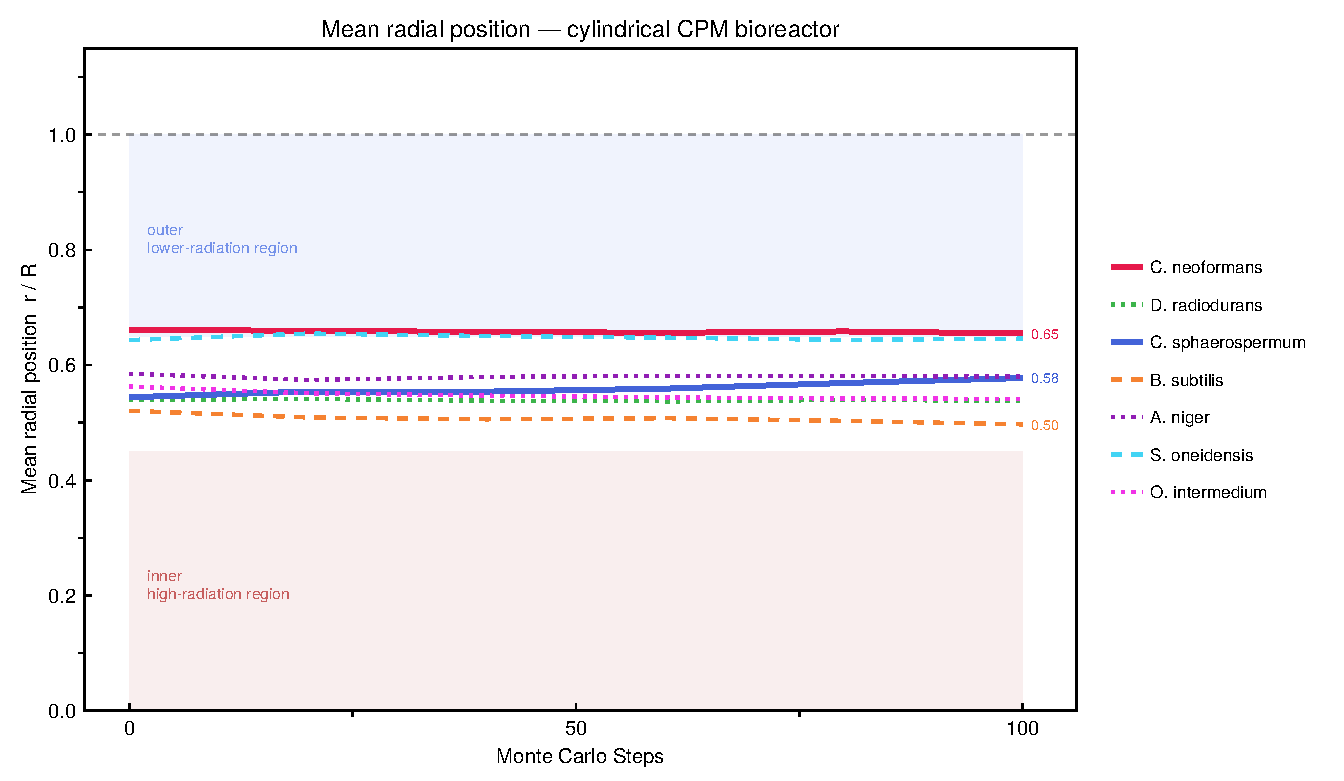
\includegraphics[width=0.91\linewidth]{fig1_radial_stratification}
\caption{Mean radial position of the seven parcel classes over 100~MCS in the coupled CPM run.
Shaded bands identify the inner high-radiation and outer lower-radiation regions of the imposed
field; they do not assert biological niches. The displayed separation is a single-seed diagnostic
and is not clearly separated from the approximate seeding null at the present parcel count.}
\label{fig:radial}
\end{figure}

\subsection{Melanin-Field Diagnostic}

The dimensionless melanin field increases over the 100-MCS run for all three producer classes
(Figure~\ref{fig:melanin}). \textit{C.~sphaerospermum} reaches the largest final field value,
$M=1.44$, followed by \textit{C.~neoformans} and \textit{A.~niger}. The ordering follows the
hand-specified production scales; these field values have no calibration to a physical melanin mass
or concentration.

\begin{figure}[htbp]
\centering
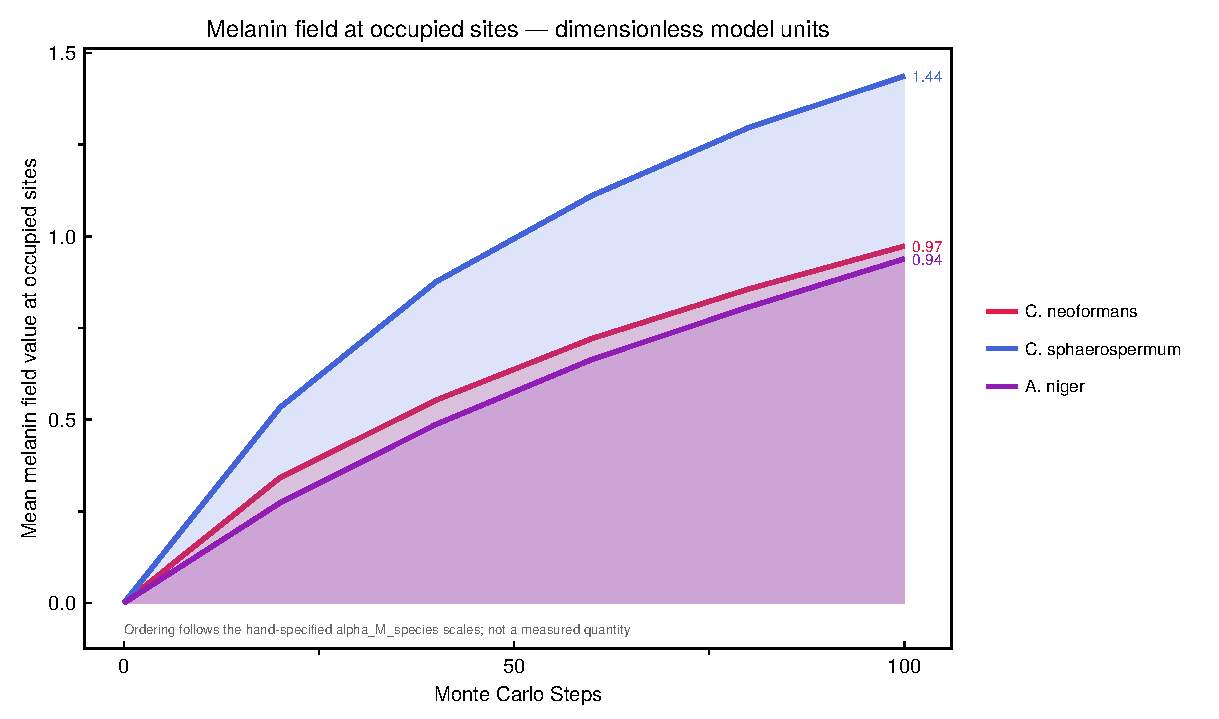
\includegraphics[width=0.85\linewidth]{fig2_melanin_accumulation}
\caption{Mean melanin field at occupied sites for the three producer classes. Values are
dimensionless model units; the sign and scale are uncalibrated and should not be interpreted as
measured melanin mass or radiation-derived energy production.}
\label{fig:melanin}
\end{figure}

\subsection{Radiodialysis Numerical Diagnostic}

The R and Julia radiodialysis implementations solve the same reaction--diffusion system with
independent time integrators. In the reported Julia run, membrane integrity decreases to
$m=0.779$ and the imposed ratio $P_{\mathrm{eff}}/P_0$ reaches $e\approx2.72$ after 100~MCS
(Figure~\ref{fig:membrane}). The latter is exact by construction from the chosen constants rather
than a fitted response. No physical MCS-to-second mapping exists, the dose-rate input is a
placeholder, and the radial coordinate is not calibrated to centimetres; these quantities are
therefore dimensionless diagnostics.

At the final snapshot, the wall concentration is approximately
$c(R,t)=0.87\,c_{\mathrm{ext}}$, while the unweighted mean over radial nodes is about
$0.024\,c_{\mathrm{ext}}$ (Figure~\ref{fig:contaminant}). The low interior value indicates limited
penetration from an initially contaminant-free interior, not depletion of a pre-existing inventory.
Because the radial biomass profile is averaged before use and site occupancy is passed where the
rate law expects mass concentration, this path remains blocked from physical interpretation.

\begin{figure}[htbp]
\centering
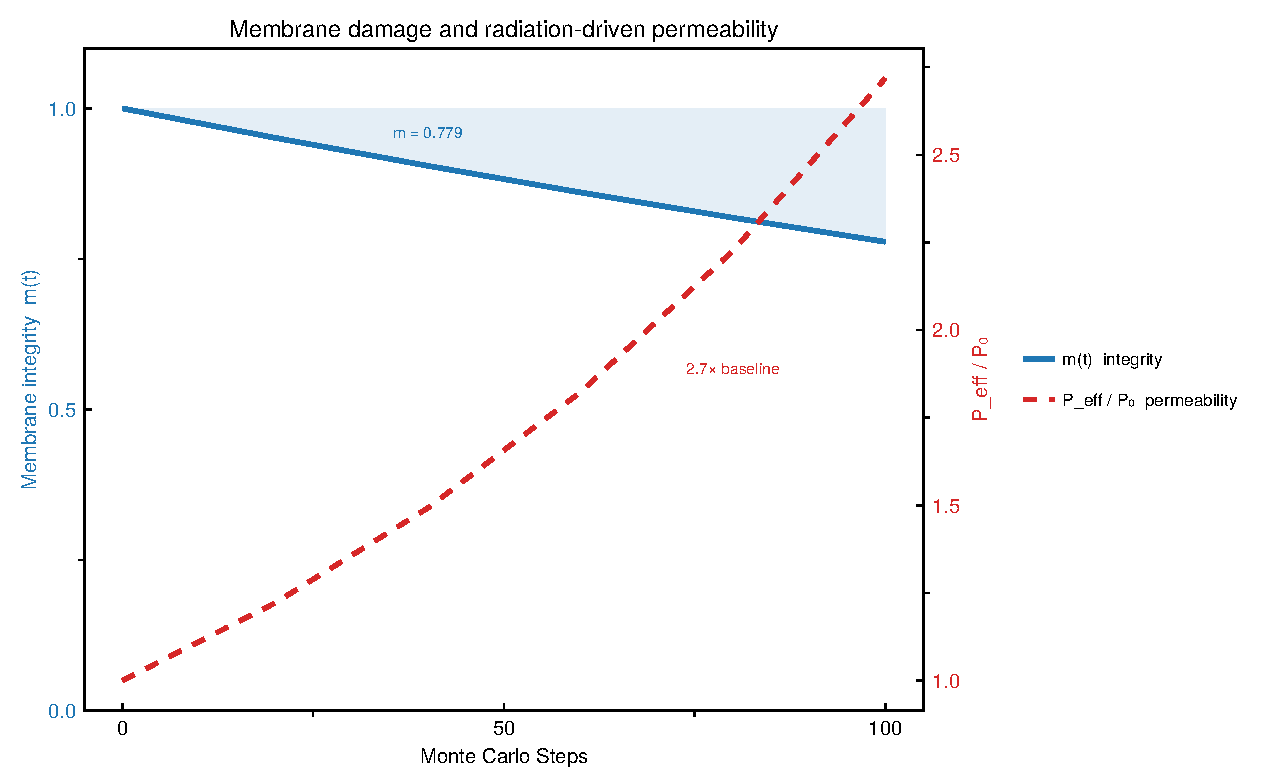
\includegraphics[width=0.88\linewidth]{fig3_membrane_transport}
\caption{Independent imposed laws for membrane integrity $m(t)$ and normalised permeability
$P_{\mathrm{eff}}(t)/P_0$ over 100~MCS. The horizontal axis is not calibrated time, and the two
curves are not a closed membrane-feedback law.}
\label{fig:membrane}
\end{figure}

\begin{figure}[htbp]
\centering
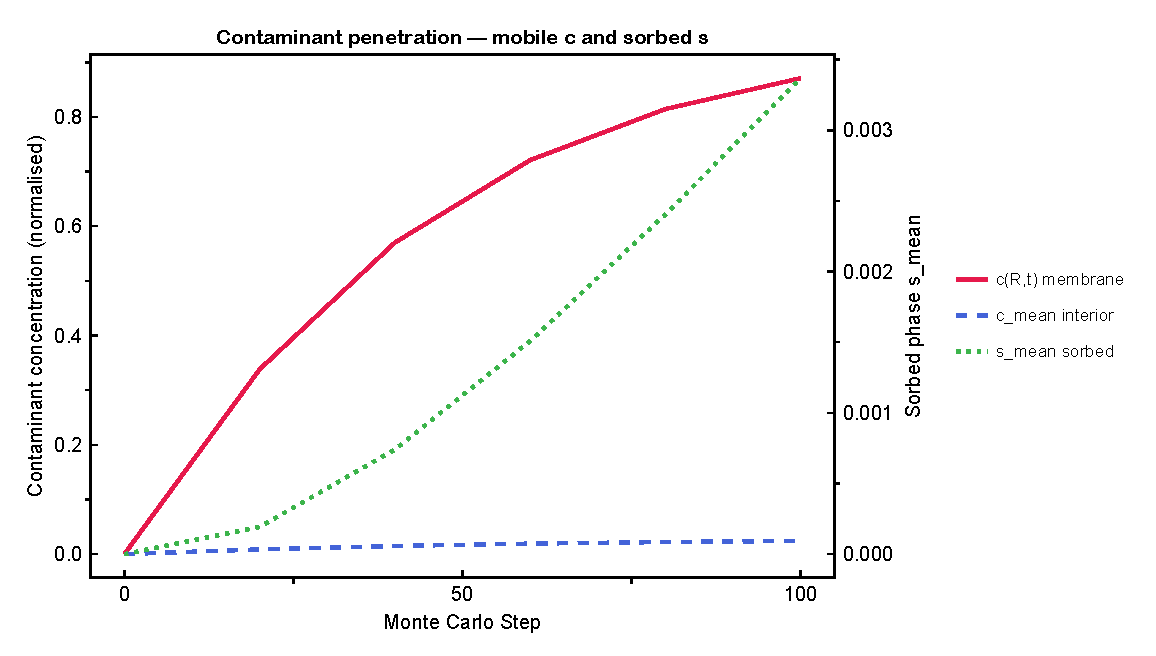
\includegraphics[width=0.88\linewidth]{fig4_contaminant_penetration}
\caption{Dimensionless mobile and sorbed contaminant diagnostics over 100~MCS. The near-zero
interior mean reflects limited penetration from the initially clean interior and must not be read as
percentage removal. The sorbed phase uses its own display scale.}
\label{fig:contaminant}
\end{figure}

\subsection{Synthetic One-Way CPM--OpenMC Integration}

The one-way transport path executed end to end under an explicitly synthetic, non-calibrating
reference system. A CPM snapshot was converted to an OpenMC biofilm-cylinder model; photon heating
was normalised with constructive-solid-geometry material volumes; per-source dose was converted to a
dose-rate field under a synthetic source rate; and the field was returned to Julia and attributed to
cell, lineage and generation labels. Orientation probes and conservation checks passed across the
exchange boundary. The run stopped before any physical dose changed the Hamiltonian, melanin,
membrane state or CPM clock. This validates the implementation path, not the physical target.

% ---- 7. Discussion -------------------------------------------
\section{Discussion}
\label{sec:discussion}

\subsection{What the Implemented Models Establish}

The implemented programs support a narrower conclusion than the full PSDE specification. The
Langevin models demonstrate stochastic spatial grouping under chosen drift and interaction rules;
they do not demonstrate radiation-enhanced growth or survival. The CPM term audit establishes that,
within its radiation-derived pathway, the melanin term exceeds the direct species-specific
radiation term by about an order of magnitude in $\Delta H$ ($9.6$), not by several. The single-seed radial output does not establish a
radiotropic pattern, because its direction conflicts with the direct coefficient and its magnitude
is not separated from the seeding null. The radiodialysis solvers establish a reproducible numerical
solution of the stated semi-discrete equations, but the coupled Julia path does not yet possess a
valid physical unit contract.

\subsection{Phenotype Boundary}

Radiotropism, radiotrophy and radioresistance refer to different observables. The present CPM can
represent only directional redistribution in a spatial field. It cannot test radiotrophy because it
has no biomass-growth process, and it cannot test radioresistance because it has no dose-dependent
survival process. The published $D_{10}$ and LD$_{90}$ measurements in
Table~\ref{tab:params} remain biologically informative, but using them to set a tropism coefficient
is a declared modelling analogy rather than a calibration of the phenotype they measured.

Melanisation is likewise not a universal proxy for either radiotrophy or survival. The literature
contains organism-, genotype-, substrate- and radiation-modality-specific effects, including
isogenic comparisons with little or no detectable pigmentation advantage. In the present CPM,
melanin is best understood as an internal model field whose coupling dominates the direct radiation
term; its physical mass, chemistry and radiobiological response remain uncalibrated.

\subsection{Implications for Bioremediation and Transport Modelling}

The one-way OpenMC foundation changes what can be tested next. Once a physically measured lattice
pitch, hydrated density, water fraction, elemental composition, membrane geometry and source model
are supplied, the same snapshot-to-dose path can evaluate whether plausible material-state changes
alter the local radiation field beyond transport and calibration uncertainty. That offline
counterfactual question is logically prior to online biological feedback: if plausible material
changes are transport-invisible, an expensive two-way coupling is not justified.

The current membrane equations do not yet support that loop. Membrane integrity and permeability
are independent imposed laws, and the radiodialysis uptake term receives occupancy fractions where
mass concentration is required. Fixed-membrane one-way dosimetry is still meaningful once the
physical system is specified; dose-responsive membrane transport requires a separate constitutive
and experimental programme.

The regime in which those inputs are obtainable is not the one this paper's motivating sites
occupy. Section~\ref{sec:planned_feedback} put the gap at about ten orders of magnitude: a
reactor irradiation delivers of order $\mathrm{Gy}\,\mathrm{min}^{-1}$ and the environmental
settings cited in Section~\ref{sec:intro} are closer to $\mathrm{mGy}\,\mathrm{yr}^{-1}$, so a sensitivity
constant calibrated in one is not transferable to the other. Engineered nuclear facilities lie
between them, and biofilms are documented there. Sarr\'{o} et al.\ submerged a bioreactor
carrying stainless steel and titanium coupons in a spent nuclear fuel pool at a Spanish nuclear
power plant, characterised the biofilm that developed on both materials, and measured its
radioactivity by gamma-ray spectrometry: the biofilms retained radionuclides from the pool water,
$^{60}$Co in particular \cite{sarro2007}. Karley et al.\ isolated six bacterial species from
spent-fuel-pool water with $D_{10}$ values from 248~Gy to 2~kGy and biofilm-forming capability,
and reported biofilm-mediated Co and Ni removal up to 3.8~$\mu$g per mg of biomass
\cite{karley2018}; a later study of the same isolates --- among them \textit{B.\ subtilis}, one
of the seven modelled here --- found that dead biomass also removed both ions, which is what a
sorption rather than a metabolic mechanism predicts \cite{karley2023}.

We record this as an observation about regime and available inputs, not as a proposed deployment.
Three quantities the offline counterfactual requires --- a bounded geometry, a characterised
source, and a measurable metal inventory in the biofilm --- are ordinarily available in such a
facility and are not available at a contaminated field site. What this framework would compute
there is the dose a biofilm on a surface receives and whether its presence perturbs the local
field: the same one-way question posed above, with its inputs supplied rather than assumed.
Whether the perturbation is large enough to matter is an empirical question, and nothing in this
paper answers it. The model is unchanged by the observation; only the setting in which its inputs
could be measured is.

\subsection{Limitations and Future Directions}
\label{sec:limitations}

\paragraph{Structural model limits.}
Growth, survival, directed hyphal elongation, phase-locking, horizontal gene transfer, and
viscoelastic mechanics are absent from the executed simulations. They cannot be recovered by fitting
new coefficients to the present state variables. Adding baseline growth and death is the minimum
model revision required before radiotrophy or radioresistance can be fitted. For directed hyphal
elongation specifically, Section~\ref{sec:radiotrophy_status} names the adaptable machinery ---
a Neighbour-Sensing- or VSC-style tip-growth term \cite{meskauskas2004,bartnickigarcia1989} ---
rather than an unbounded open problem.

Fluid flow and advection are absent as well, and the relation between these absences is more
informative than a longer list would be. Flow reaches morphology through mechanics, so its
absence is downstream of the missing mechanics rather than a separate gap; and a model with
no growth generates no growth-induced stress for mechanics to act on, so the mechanical gap
is in turn downstream of the growth one. The three are better read as one structural absence
under three names than as three independent items. What that costs is stated rather than
implied: this model has none of the three routes named above, and its spatial output is
therefore directional redistribution of parcels in an imposed field rather than a morphology.
Whether those three exhaust the routes is a question about the literature and not one this
model answers.
External review has argued that growth-induced stress is the dominant morphogen in still
conditions; that claim is literature this work has not verified, is recorded as such in
\texttt{docs/research/external\_reviews\_2026-08-31\_redteam.md}, and nothing here
depends on it.

\paragraph{Identifiability.}
Only the product of the melanin-production scale and the melanin-coupling scale reaches the CPM
acceptance dynamics. Those parameters cannot be estimated separately from the same output without
an independent measurement or reparameterisation.

\paragraph{Physical calibration.}
No value in Table~\ref{tab:params} is fitted to the target system. Lattice pitch, wet bulk density,
water fraction, closed hydrated elemental composition, seconds per MCS, source activity, and
biological response normalisations remain unset. Public datasets can exercise parts of the
acquisition pipeline, but no located source provides a paired target-compatible combination of
calibrated three-dimensional morphology, wet and dry mass with matched blanks, elemental
composition, and characterised radiation exposure \cite{audit2026}.

\paragraph{Numerical resolution and uncertainty.}
The physical dose effect must be evaluated over independent transport replicates, declared mesh and
ray-tracing convergence axes, correlated calibration draws, and explicit model-form scenarios.
Numerical resolution is a bound to be reduced, not a random parameter to be averaged into the
physical posterior. The scientific effect threshold must be declared prospectively before target
feedback results are inspected.

\paragraph{Experimental next step.}
A target Reference D campaign should pair calibrated 3-D biomass imaging with matched wet/dry
measurements, hydrated-volume support, abiotic blanks, closed wet-bulk composition, exact strain
identities, and a characterised irradiation geometry. Culturing must begin only after the relevant
facility has issued strain- and protocol-specific biosafety approval. The measured configuration can
then support a biofilm-specific transport-resolution study, a one-way physical dose calculation,
and finally the scientific offline feedback gate.

% ---- 8. Conclusion -------------------------------------------
\section{Conclusion}

This study separates a broad mathematical proposal from the smaller set of simulations that were
actually executed. The active CPM represents seven species as computational biomass parcels and
contains adhesion, volume, radiation and melanin terms. At the shipped constants, the melanin term
is the dominant radiation-derived contribution to Metropolis acceptance, exceeding the direct
species-specific radiation term by about an order of magnitude in $\Delta H$ rather than rendering it
negligible. The resulting
single-seed radial pattern is diagnostic rather than established: it is opposite to the direct-term
direction and is not separated from the seeding null at six parcels per species.

The implemented phenotype is radiotropism alone. Radiotrophy and radioresistance remain outside the
current state space because the model has no biomass growth or dose-dependent survival. The
radiodialysis solver is numerically defined but physically blocked by its occupancy-to-mass and
membrane-law inconsistencies. In contrast, the synthetic one-way CPM--OpenMC path has executed
through geometry export, photon transport, exact-volume dose normalisation, coordinate transfer and
label attribution while remaining explicitly non-calibrating.

The immediate scientific requirement is therefore measurement rather than additional architectural
coupling: paired three-dimensional morphology, wet and dry mass, water fraction, closed hydrated
composition, source characterisation and a prospective effect threshold. Those inputs would permit
a measured Reference D configuration, a biofilm-specific resolution study, and an offline test of
whether plausible biological material changes are large enough to justify any online feedback.

\section*{Software and Data Availability}
All source code, configuration schemas, tests, provenance ledgers, and figure-generation materials
are available in the public repository at
\url{https://github.com/aurascoper/Biofilms}. Version 1.0 was prepared against repository
revision \texttt{c7539a9}; this revision is prepared against \texttt{4d8a5f8}. Each names the
parent of the commit that adds it, because a document cannot cite the commit that contains it. No new biological specimens or experimental measurements were generated.
Third-party public datasets are cited by their original records and are not redistributed as target
calibration data.

Readers should note that the repository has continued past this revision, and that several
numerical results published in it were subsequently corrected by the project's own review: a
false-positive control that could not fail was replaced, a squared difference reported as a
variance was relabelled, an unprovenanced sensitivity table was withdrawn and re-measured, and
one synthetic-gate verdict was withdrawn as not resolution-converged. The corrections are
recorded in \texttt{data/claims\_ledger.csv} and in \texttt{docs/calibration/}.

\emph{Correction, version 1.1: Figures 1 and 2 have been replaced.} The versions distributed with
version 1.0 carried claims inside the images that the surrounding text retracts. Figure 2
annotated two species as ``radiotrophic (melanin-mediated energy gain)'' beneath a caption
disowning radiation-derived energy production and against
Section~\ref{sec:radiotrophy_status}; Figure~1 labelled a shaded band a ``radiotrophic niche'',
and labelled it on the wrong side, since the imposed field is maximal on the axis. Three further
in-plot strings asserted findings the text does not support: a title reading ``radial
stratification'' where Section~\ref{sec:discussion} reports a single-seed diagnostic not separated from the seeding
null, a title attributing melanin accumulation to radiation-driven production, and an annotation
asserting drift toward the source when the run's own ordering runs the other way. No numerical
value in either figure changed --- the underlying run is the same, and the mean radial positions
and melanin values quoted in the captions are reproduced exactly --- and no other figure was
regenerated. Figure~4 still carries a ``per cent depleted'' label that should read
non-penetration, and is not regenerated here: its quantities are downstream of the gated biomass
basis. Figure~3 is not --- it plots $m(t)$ and $P_{\mathrm{eff}}/P_0$, neither of which reads that
basis --- and it has now been rebuilt; see the version 1.2 note below. The defect was that the
figure generator had been corrected two weeks earlier and the committed images had not, with no
check able to detect the difference; this is recorded as \texttt{FIG-01} to \texttt{FIG-07} in the
claims ledger.

\emph{Correction, version 1.2: two items, one numerical and one in an image.}
Section~\ref{sec:cpm_term_magnitudes} previously bounded the acceptance-favouring contribution of
$\Delta H_{\mathrm{rad}}$ at $5\times10^{-5}$ and inferred from that bound that the term deciding
no accepted move was analytically expected rather than an under-sampling artifact. The bound was
wrong by a factor of $1.5\times10^{3}$: it enumerated only the source-gains-a-site role, and a
positively signed species vacating a site favours acceptance by up to $7.5\times10^{-2}$. A second
pass over the same paragraph, also in review, found that the replacement bound was still stated over
\emph{species} when the quantity is an extremum over source/target \emph{pairings}: a copy between
two occupied parcels carries both roles, so the reach is $7.505\times10^{-2}$ and
$\max_s|\beta_{s,\mathrm{ion}}|$ is not a bound on it. The two values differ by $0.067\%$ and the
larger is attained in a shipped configuration. The fraction of evaluated proposals carrying
$\Delta H_{\mathrm{rad}} < -5\times10^{-5}$ is likewise restated as $26.7\%$ over the three runs of
Table~\ref{tab:decided_moves}; the $29.8\%$ first written here came from a run this paper did not
identify, which is the same defect as \texttt{PP-62-11} and is why the configuration is now named in
the sentence. \texttt{tests/prose\_bounds.jl} recomputes the bound from the shipped coefficients and
fails on either withdrawn form.
Table~\ref{tab:term_magnitudes} gains the missing row and the paragraph beneath
Table~\ref{tab:decided_moves} is rewritten. \textbf{Two published numbers move.} The count of moves
for which the direct radiation term was solely decisive is one of 206\,042, not zero --- seed 44
carries one --- and the number that removing $\Delta H_{\mathrm{rad}}$ alone would reverse is
sixteen, against $0.26$ predicted under the withdrawn bound and $16.7$ under the corrected one. The
remaining entries of Table~\ref{tab:decided_moves} were re-measured and reproduce exactly; that is
a statement about those entries and not about any other result in this paper. Recorded as
\texttt{PP-62-04} and \texttt{PP-62-09} to \texttt{PP-62-11} in the claims ledger; raised in review
by Codex on pull request \#23. Figure~3 has separately been rebuilt to remove an in-plot
``50~Gy cumulative'' annotation that the generator dropped on 14 August 2026 and the committed
artifact kept, and to separate two labels that had been printing on top of one another; no value in
it changed.

\section*{Ethics, Biosafety, and Regulatory Statement}
This manuscript reports software development, computational simulation, code audit, and analysis of
published or publicly available information. It involved no human participants, vertebrate animals,
live microbial culture, recombinant or synthetic nucleic-acid experiment, or physical
ionising-radiation experiment. No institutional human-subject, animal-use, biosafety, or radiation-use approval was required
for the work reported here. Any future target culture or
irradiation campaign will begin only after strain-, protocol-, facility- and source-specific
institutional approvals have been issued; no such campaign or approval is claimed in this
manuscript.

One organism named here requires a nomenclature note, because the name it is published under is
no longer the name a laboratory would receive it as. \textit{Ochrobactrum intermedium} was
reclassified into \textit{Brucella} on genomic grounds \cite{hordt2020}, the combination
\textit{Brucella intermedia} was validly published the same year \cite{oren2020}, and NCBI
Taxonomy serves taxon 94625 as \textit{Brucella intermedia} with \textit{Ochrobactrum
intermedium} retained as a synonym and a lineage reading \texttt{Brucellaceae; Brucella/}
\texttt{Ochrobactrum group; Brucella}. The consequence is operational rather than taxonomic: CDC's
laboratory update of 19 December 2022 records that the reclassification is reflected in the rapid
identification systems clinical laboratories use, and directs that organisms identified as
\textit{Brucella} be handled in a Class II biosafety cabinet and that presumptive isolates be
referred to a state public health laboratory \cite{cdc2022}. That same notice designates the
former \textit{Ochrobactrum} species non-brucellosis-causing.

We state the record and not a determination. Containment level, select-agent status and
procurement clearance follow the individual strain, are the responsibility of the institution
that issues them, and are outside what a computational study can establish; this manuscript
asserts none of them. Two facts are recorded because they bear on anyone reading this as a
procurement plan: no culture-collection accession for AM7 was located in any repository searched,
so the strain may be unobtainable; and the repository's own research record carries the
determination as unresolved, with procurement held pending it. Both names are carried on every
record here for the same reason the \textit{Wangiella}/\textit{Exophiala} mapping is carried
--- a search under one name does not return the other.

% ---- References ---------------------------------------------
\begin{thebibliography}{61}

\bibitem{radcell2021}
Liu, R., Higley, K.A., Swat, M.H., Chaplain, M.A.J., Powathil, G.G., Glazier, J.A. (2021).
Development of a coupled simulation toolkit for computational radiation biology based on
Geant4 and CompuCell3D.
\textit{Physics in Medicine \& Biology}, 66(4), 045026.
\url{https://doi.org/10.1088/1361-6560/abd4f9}

\bibitem{garciagarcia2024}
Garc\'{i}a Garc\'{i}a, O.R., Ortiz, R., Moreno-Barbosa, E., D-Kondo, N., Faddegon, B.,
Ramos-M\'{e}ndez, J. (2024).
TOPAS-Tissue: a framework for the simulation of the biological response to ionizing radiation
at the multi-cellular level.
\textit{International Journal of Molecular Sciences}, 25(18), 10061.
\url{https://doi.org/10.3390/ijms251810061}

\bibitem{cogno2024}
Cogno, N., Bauer, R., Durante, M. (2024).
Mechanistic model of radiotherapy-induced lung fibrosis using coupled 3D agent-based and
Monte Carlo simulations.
\textit{Communications Medicine}, 4, 16.
\url{https://doi.org/10.1038/s43856-024-00442-w}

\bibitem{meskauskas2004}
Me\v{s}kauskas, A., Fricker, M.D., Moore, D. (2004).
Simulating colonial growth of fungi with the Neighbour-Sensing model of hyphal growth.
\textit{Mycological Research}, 108(11), 1241--1256.
\url{https://doi.org/10.1017/S0953756204001261}

\bibitem{bartnickigarcia1989}
Bartnicki-Garcia, S., Hergert, F., Gierz, G. (1989).
Computer simulation of fungal morphogenesis and the mathematical basis for hyphal
(tip) growth.
\textit{Protoplasma}, 153, 46--57.
\url{https://doi.org/10.1007/BF01322464}

\bibitem{shuryak2014}
Shuryak, I., Bryan, R.A., Nosanchuk, J.D., Dadachova, E. (2014).
Mathematical modeling predicts enhanced growth of X-ray irradiated pigmented fungi.
\textit{PLoS ONE}, 9(1), e85561.
\url{https://doi.org/10.1371/journal.pone.0085561}

\bibitem{zhdanova2000}
Zhdanova, N.N., Zakharchenko, V.A., Vember, V.V., Nakonechnaya, L.T. (2000).
Fungi from Chernobyl: mycobiota of the inner regions of the containment structures of the
damaged nuclear reactor.
\textit{Mycological Research}, 104(12), 1421--1426.
\url{https://doi.org/10.1017/S0953756200002756}

\bibitem{dadachova2007}
Dadachova, E., Bryan, R.A., Huang, X., Moadel, T., Schweitzer, A.D., Aisen, P.,
Nosanchuk, J.D., Casadevall, A. (2007).
Ionizing radiation changes the electronic properties of melanin and enhances the growth of
melanized fungi.
\textit{PLoS ONE}, 2(5), e457.
\url{https://doi.org/10.1371/journal.pone.0000457}

\bibitem{dadachova2008}
Dadachova, E., Casadevall, A. (2008).
Ionizing radiation: how fungi cope, adapt, and exploit with the help of melanin.
\textit{Current Opinion in Microbiology}, 11(6), 525--531.
\url{https://doi.org/10.1016/j.mib.2008.09.013}

\bibitem{shunk2022}
Shunk, G.K., Gomez, X.R., Kern, C., Averesch, N.J.H. (2022).
Cultivation of the dematiaceous fungus \textit{Cladosporium sphaerospermum} aboard the
International Space Station and effects of ionizing radiation.
\textit{Frontiers in Microbiology}, 13, 877625.
\url{https://doi.org/10.3389/fmicb.2022.877625}

\bibitem{slade2011}
Slade, D., Radman, M. (2011).
Oxidative stress resistance in \textit{Deinococcus radiodurans}.
\textit{Microbiology and Molecular Biology Reviews}, 75(1), 133--191.
\url{https://doi.org/10.1128/MMBR.00015-10}

\bibitem{daly2009}
Daly, M.J. (2009).
A new perspective on radiation resistance based on \textit{Deinococcus radiodurans}.
\textit{Nature Reviews Microbiology}, 7(3), 237--245.
\url{https://doi.org/10.1038/nrmicro2073}

\bibitem{daly2010}
Daly, M.J., et al. (2010).
Small-molecule antioxidant proteome-shields in \textit{Deinococcus radiodurans}.
\textit{PLoS ONE}, 5(9), e12570.
\url{https://doi.org/10.1371/journal.pone.0012570}

\bibitem{wanner1986}
Wanner, O., Gujer, W. (1986).
A multispecies biofilm model.
\textit{Biotechnology and Bioengineering}, 28(3), 314--328.
\url{https://doi.org/10.1002/bit.260280304}

\bibitem{xavier2005}
Xavier, J.B., Picioreanu, C., van Loosdrecht, M.C.M. (2005).
A framework for multidimensional modelling of activity and structure of multispecies biofilms.
\textit{Environmental Microbiology}, 7(8), 1085--1103.
\url{https://doi.org/10.1111/j.1462-2920.2005.00787.x}

\bibitem{lardon2011}
Lardon, L.A., et al. (2011).
iDynoMiCS: next-generation individual-based modelling of biofilms.
\textit{Environmental Microbiology}, 13(9), 2416--2434.
\url{https://doi.org/10.1111/j.1462-2920.2011.02414.x}

\bibitem{sonner2015}
Rahman, K.A., Sudarsan, R., Eberl, H.J. (2015).
A mixed-culture biofilm model with cross-diffusion.
\textit{Bulletin of Mathematical Biology}, 77(11), 2086--2124.
\url{https://doi.org/10.1007/s11538-015-0117-1}
% CORRECTED 2026-08-31. The entry previously here had wrong bibliographic data,
% a DOI resolving to an unrelated paper, and was the wrong paper for the
% cross-diffusion claim it was cited for. The withdrawn fields are recorded in
% data/claims_ledger.csv, row PP-REF-01 (verdict delete) -- deliberately NOT
% repeated here, so the withdrawn DOI exists in the recording layer only and
% cannot be copied out of the manuscript.

\bibitem{diele2015}
Diele, F., Marangi, C. (2020).
Geometric numerical integration in ecological modelling.
\textit{Mathematics}, 8(1), 25.
\url{https://doi.org/10.3390/math8010025}
% CORRECTED 2026-08-31. EVERY FIELD of the previous entry was wrong -- authors,
% year, journal, volume, pages -- and its DOI resolved to an unrelated
% quadratic-programming paper. Two authors, not three; the body citation was
% updated to match. The withdrawn fields are in data/claims_ledger.csv, row
% PP-REF-02 (verdict delete), and are deliberately not repeated here.

\bibitem{kuramoto1984}
Kuramoto, Y. (1984).
\textit{Chemical Oscillations, Waves, and Turbulence}.
Springer-Verlag, Berlin.
\url{https://doi.org/10.1007/978-3-642-69689-3}

\bibitem{acebron2005}
Aceb\'r\'on, J.A., Bonilla, L.L., P\'erez Vicente, C.J., Ritort, F., Spigler, R. (2005).
The Kuramoto model: a simple paradigm for synchronization phenomena.
\textit{Reviews of Modern Physics}, 77(1), 137--185.
\url{https://doi.org/10.1103/RevModPhys.77.137}

\bibitem{campillo2017}
Voulgarelis, D., Velayudhan, A., Smith, F. (2018).
Stochastic analysis of a full system of two competing populations in a chemostat.
\textit{Chemical Engineering Science}, 175, 424--444.
% CORRECTED 2026-08-31 per claims_ledger PP-REF-03, which holds the withdrawn wording.
% The journal and volume were right; the authors, year, title and pages were not.
% The key is left as campillo2017 so the citation sites need no edit.
\url{https://doi.org/10.1016/j.ces.2017.10.016}

\bibitem{heidelberg2002}
Heidelberg, J.F., et al. (2002).
Genome sequence of the dissimilatory metal ion-reducing bacterium
\textit{Shewanella oneidensis}.
\textit{Nature Biotechnology}, 20(11), 1118--1123.
\url{https://doi.org/10.1038/nbt749}

\bibitem{veeramani2011}
Veeramani, H., et al. (2011).
Products of abiotic U(VI) reduction by biogenic magnetite and vivianite.
\textit{Geochimica et Cosmochimica Acta}, 75(9), 2512--2528.
\url{https://doi.org/10.1016/j.gca.2011.02.024}

\bibitem{shukla2020}
Shukla, A., Parmar, P., Goswami, D., Patel, B., Saraf, M. (2020).
Characterization of novel thorium tolerant \textit{Ochrobactrum intermedium} AM7.
\textit{Journal of Hazardous Materials}, 388, 122047.
\url{https://doi.org/10.1016/j.jhazmat.2020.122047}

\bibitem{sarro2007}
Sarr\'{o}, M. I., Garc\'{i}a, A. M., Moreno, D. A., Montero, F. (2007).
Development and characterization of biofilms on stainless steel and titanium in spent nuclear
fuel pools.
\textit{Journal of Industrial Microbiology \& Biotechnology}, 34(6), 433--441.
\url{https://doi.org/10.1007/s10295-007-0215-7}

\bibitem{karley2018}
Karley, D., Shukla, S. K., Rao, T. S. (2018).
Isolation and characterization of culturable bacteria present in the spent nuclear fuel pool
water.
\textit{Environmental Science and Pollution Research}, 25(21), 20518--20526.
\url{https://doi.org/10.1007/s11356-017-0376-5}

\bibitem{karley2023}
Karley, D., Shukla, S. K., Rao, T. S. (2023).
Sequestration of cobalt and nickel by biofilm forming bacteria isolated from spent nuclear fuel
pool water.
\textit{Environmental Monitoring and Assessment}, 195(6), 731.
\url{https://doi.org/10.1007/s10661-023-11266-x}

\bibitem{hordt2020}
H\"{o}rdt, A., Garc\'{i}a L\'{o}pez, M., Meier-Kolthoff, J. P., Schleuning, M., Weinhold, L.-M.,
Tindall, B. J., Gronow, S., Kyrpides, N. C., Woyke, T., G\"{o}ker, M. (2020).
Analysis of 1,000+ type-strain genomes substantially improves taxonomic classification of
\textit{Alphaproteobacteria}.
\textit{Frontiers in Microbiology}, 11, 468.
\url{https://doi.org/10.3389/fmicb.2020.00468}

\bibitem{oren2020}
Oren, A., Garrity, G. M. (2020).
List of new names and new combinations previously effectively, but not validly, published.
\textit{International Journal of Systematic and Evolutionary Microbiology}, 70(7), 4043--4049.
\url{https://doi.org/10.1099/ijsem.0.004244}

\bibitem{cdc2022}
Centers for Disease Control and Prevention (2022).
Lab update: reclassification of \textit{Ochrobactrum} species into the \textit{Brucella} genus.
Laboratory Outreach Communication System, 19 December 2022.
\url{https://www.cdc.gov/locs/2022/12-19-2022-Lab-Update-Reclassification_Ochrobactrum_species_Brucella_genus.html}

\bibitem{wright1932}
Wright, S. (1932).
The roles of mutation, inbreeding, crossbreeding and selection in evolution.
\textit{Proceedings of the Sixth International Congress of Genetics}, 1, 356--366.

\bibitem{kauffman1989}
Kauffman, S.A., Weinberger, E.D. (1989).
The NK model of rugged fitness landscapes.
\textit{Journal of Theoretical Biology}, 141(2), 211--245.
\url{https://doi.org/10.1016/S0022-5193(89)80019-0}

\bibitem{berg1993}
Berg, H.C. (1993).
\textit{Random Walks in Biology}.
Princeton University Press.

\bibitem{guttenplan2013}
Guttenplan, S.B., Shaw, S., Kearns, D.B. (2013).
The cell biology of peritrichous flagella in \textit{Bacillus subtilis}.
\textit{Molecular Microbiology}, 87(1), 211--229.
\url{https://doi.org/10.1111/mmi.12103}

\bibitem{nicholson2000}
Nicholson, W.L., et al. (2000).
Resistance of \textit{Bacillus} endospores to extreme terrestrial and extraterrestrial
environments.
\textit{Microbiology and Molecular Biology Reviews}, 64(3), 548--572.
\url{https://doi.org/10.1128/MMBR.64.3.548-572.2000}

\bibitem{turick2011}
Turick, C.E., et al. (2011).
Gamma radiation interacts with melanin to alter its oxidation-reduction potential and
results in electric current production.
\textit{Bioelectrochemistry}, 82(1), 69--73.
\url{https://doi.org/10.1016/j.bioelechem.2011.04.009}

\bibitem{robertson2012}
Robertson, K.L., et al. (2012).
Adaptation of the black yeast \textit{Wangiella dermatitidis} to ionizing radiation.
\textit{PLoS ONE}, 7(11), e48674.
\url{https://doi.org/10.1371/journal.pone.0048674}

\bibitem{malo2018} 
Malo, M.E., Bryan, R.A., Shuryak, I., Dadachova, E. (2018).
Morphological changes in melanized and non-melanized \textit{Cryptococcus neoformans} cells
post exposure to sparsely and densely ionizing radiation demonstrate protective effect of
melanin.
\textit{Fungal Biology}, 122(6), 449--456.
\url{https://doi.org/10.1016/j.funbio.2017.08.010}

\bibitem{blasius1999}
Blasius, B., Huppert, A., Stone, L. (1999).
Complex dynamics and phase synchronization in spatially extended ecological systems.
\textit{Nature}, 399, 354--359.
\url{https://doi.org/10.1038/20676}

\bibitem{alpkvist2007}
Alpkvist, E., Klapper, I. (2007).
A multidimensional multispecies continuum model for heterogeneous biofilm development.
\textit{Bulletin of Mathematical Biology}, 69(2), 765--789.
\url{https://doi.org/10.1007/s11538-006-9168-7}

\bibitem{eberl2001}
Eberl, H.J., Parker, D.F., van Loosdrecht, M.C.M. (2000).
A new deterministic spatio-temporal continuum model for biofilm development.
\textit{Journal of Theoretical Medicine} (now \textit{Computational and Mathematical
Methods in Medicine}), 3(3), 161--175.
\url{https://doi.org/10.1080/10273660108833072}

\bibitem{hairer2006}
Hairer, E., Lubich, C., Wanner, G. (2006).
\textit{Geometric Numerical Integration}, 2nd ed.
Springer-Verlag.
\url{https://doi.org/10.1007/3-540-30666-8}

\bibitem{khajo2011}
Khajo, A., et al. (2011).
Protection of melanized \textit{Cryptococcus neoformans} from lethal dose gamma irradiation.
\textit{PLoS ONE}, 6(9), e25092.
\url{https://doi.org/10.1371/journal.pone.0025092}

\bibitem{casadevall2017}
Casadevall, A., et al. (2017).
Melanin, radiation, and energy transduction in fungi.
\textit{Microbiology Spectrum}, 5(2), FUNK-0037-2016.
\url{https://doi.org/10.1128/microbiolspec.FUNK-0037-2016}

\bibitem{graner1992}
Graner, F., Glazier, J.A. (1992).
Simulation of biological cell sorting using a two-dimensional extended Potts model.
\textit{Physical Review Letters}, 69(13), 2013--2016.
\url{https://doi.org/10.1103/PhysRevLett.69.2013}

\bibitem{fox2009}
Fox, E.B., et al. (2009).
Radiation effects on Nafion$^{\circledR}$ membrane properties.
\textit{Savannah River National Laboratory Technical Report}, SRNL-STI-2009-00053.

\bibitem{lara2023}
Lara, D., et al. (2023).
Ionizing radiation effects on proton exchange membrane permeability and selectivity.
\textit{Membranes}, 13(4), 412.
\url{https://doi.org/10.3390/membranes13040412}

\bibitem{renslow2017}
Renslow, R.S., et al. (2017).
Modeling biofilm-mediated uranium immobilization in porous media.
\textit{Water Research}, 109, 120--130.
\url{https://doi.org/10.1016/j.watres.2016.11.038}

\bibitem{aydogan2022}
Aydogan Gokturk, P., Sujanani, R., Qian, J., Wang, L., Freyman, J.L., Bhatt, A.D.,
Freeman, B.D., Bhave, R., Boudouris, B.W., Phillip, W.A. (2022).
Donnan dialysis of monovalent ions across a cation exchange membrane.
\textit{Nature Communications}, 13, 5258.
\url{https://doi.org/10.1038/s41467-022-32930-9}

\bibitem{soetaert2010}
Soetaert, K., Petzoldt, T., Setzer, R.W. (2010).
Solving differential equations in R: package deSolve.
\textit{Journal of Statistical Software}, 33(9), 1--25.
\url{https://doi.org/10.18637/jss.v033.i09}

\bibitem{cortesao2020}
Cortes\~{a}o, M., et al. (2020).
Aspergillus niger spores are highly resistant to space radiation.
\textit{Frontiers in Microbiology}, 11, article 560.
(LD$_{90}$ values for N402 and the pigmentation-deficient $\Delta fwnA$ mutant MA93.1 under
X-ray, He-ion and Fe-ion exposure; open access, CC BY 4.0.)

\bibitem{sellafield2020}
Foster, L., Boothman, C., Ruiz-Lopez, S., et al. (2020).
Identification of a stable hydrogen-driven microbiome in a highly radioactive storage facility on
the Sellafield site. \textit{Frontiers in Microbiology}, 11, 587556.

\bibitem{sellafield2023}
Ruiz-Lopez, S., et al. (2023).
Identification of algal rich microbial blooms in the Sellafield Pile Fuel Storage Pond and the
application of ultrasonic treatment to control the formation of blooms.
\textit{Frontiers in Microbiology}, 14, 1261801.

\bibitem{walberg2015}
Walberg, K. (2015).
Assessment of the evidence for radiosynthesis in melanized fungi.
Undergraduate thesis, University of Wisconsin--La Crosse. \texttt{handle:1793/73406}.
(Licence not specified in the repository record. Contains no new measurement; the argument is a
closed energy budget plus a media-carbon confounder.)

\bibitem{audit2026}
Kinder, H., Faulkner, B. (2026).
Radiotrophic compatibility audit: public evidence for the radiation phenotypes of seven modelled
species. Project technical record, \texttt{docs/research/radiotrophic\_compatibility\_audit.md},
commits \texttt{904b9a4} and \texttt{a03bc32}, repository revision \texttt{c7539a9}.
(Eleven data repositories, the NCBI archives and Europe PMC searched at API level; every phenotype
label assigned from the endpoint actually measured; every unverified quantity recorded as
unverified. Four verdicts, quoted in Section~\ref{sec:radiotrophy_status}. This record populates no
parameter.)

\end{thebibliography}

\end{document}
